\documentclass[]{article}
\usepackage{lmodern}
\usepackage{amssymb,amsmath}
\usepackage{ifxetex,ifluatex}
\usepackage{fixltx2e} % provides \textsubscript
\ifnum 0\ifxetex 1\fi\ifluatex 1\fi=0 % if pdftex
  \usepackage[T1]{fontenc}
  \usepackage[utf8]{inputenc}
\else % if luatex or xelatex
  \ifxetex
    \usepackage{mathspec}
  \else
    \usepackage{fontspec}
  \fi
  \defaultfontfeatures{Ligatures=TeX,Scale=MatchLowercase}
\fi
% use upquote if available, for straight quotes in verbatim environments
\IfFileExists{upquote.sty}{\usepackage{upquote}}{}
% use microtype if available
\IfFileExists{microtype.sty}{%
\usepackage{microtype}
\UseMicrotypeSet[protrusion]{basicmath} % disable protrusion for tt fonts
}{}
\usepackage[margin=1in]{geometry}
\usepackage{hyperref}
\hypersetup{unicode=true,
            pdftitle={Assignment 5},
            pdfauthor={Angie Bouche, Tara Jagadeesh, Andrea Cheung},
            pdfborder={0 0 0},
            breaklinks=true}
\urlstyle{same}  % don't use monospace font for urls
\usepackage{color}
\usepackage{fancyvrb}
\newcommand{\VerbBar}{|}
\newcommand{\VERB}{\Verb[commandchars=\\\{\}]}
\DefineVerbatimEnvironment{Highlighting}{Verbatim}{commandchars=\\\{\}}
% Add ',fontsize=\small' for more characters per line
\usepackage{framed}
\definecolor{shadecolor}{RGB}{248,248,248}
\newenvironment{Shaded}{\begin{snugshade}}{\end{snugshade}}
\newcommand{\KeywordTok}[1]{\textcolor[rgb]{0.13,0.29,0.53}{\textbf{#1}}}
\newcommand{\DataTypeTok}[1]{\textcolor[rgb]{0.13,0.29,0.53}{#1}}
\newcommand{\DecValTok}[1]{\textcolor[rgb]{0.00,0.00,0.81}{#1}}
\newcommand{\BaseNTok}[1]{\textcolor[rgb]{0.00,0.00,0.81}{#1}}
\newcommand{\FloatTok}[1]{\textcolor[rgb]{0.00,0.00,0.81}{#1}}
\newcommand{\ConstantTok}[1]{\textcolor[rgb]{0.00,0.00,0.00}{#1}}
\newcommand{\CharTok}[1]{\textcolor[rgb]{0.31,0.60,0.02}{#1}}
\newcommand{\SpecialCharTok}[1]{\textcolor[rgb]{0.00,0.00,0.00}{#1}}
\newcommand{\StringTok}[1]{\textcolor[rgb]{0.31,0.60,0.02}{#1}}
\newcommand{\VerbatimStringTok}[1]{\textcolor[rgb]{0.31,0.60,0.02}{#1}}
\newcommand{\SpecialStringTok}[1]{\textcolor[rgb]{0.31,0.60,0.02}{#1}}
\newcommand{\ImportTok}[1]{#1}
\newcommand{\CommentTok}[1]{\textcolor[rgb]{0.56,0.35,0.01}{\textit{#1}}}
\newcommand{\DocumentationTok}[1]{\textcolor[rgb]{0.56,0.35,0.01}{\textbf{\textit{#1}}}}
\newcommand{\AnnotationTok}[1]{\textcolor[rgb]{0.56,0.35,0.01}{\textbf{\textit{#1}}}}
\newcommand{\CommentVarTok}[1]{\textcolor[rgb]{0.56,0.35,0.01}{\textbf{\textit{#1}}}}
\newcommand{\OtherTok}[1]{\textcolor[rgb]{0.56,0.35,0.01}{#1}}
\newcommand{\FunctionTok}[1]{\textcolor[rgb]{0.00,0.00,0.00}{#1}}
\newcommand{\VariableTok}[1]{\textcolor[rgb]{0.00,0.00,0.00}{#1}}
\newcommand{\ControlFlowTok}[1]{\textcolor[rgb]{0.13,0.29,0.53}{\textbf{#1}}}
\newcommand{\OperatorTok}[1]{\textcolor[rgb]{0.81,0.36,0.00}{\textbf{#1}}}
\newcommand{\BuiltInTok}[1]{#1}
\newcommand{\ExtensionTok}[1]{#1}
\newcommand{\PreprocessorTok}[1]{\textcolor[rgb]{0.56,0.35,0.01}{\textit{#1}}}
\newcommand{\AttributeTok}[1]{\textcolor[rgb]{0.77,0.63,0.00}{#1}}
\newcommand{\RegionMarkerTok}[1]{#1}
\newcommand{\InformationTok}[1]{\textcolor[rgb]{0.56,0.35,0.01}{\textbf{\textit{#1}}}}
\newcommand{\WarningTok}[1]{\textcolor[rgb]{0.56,0.35,0.01}{\textbf{\textit{#1}}}}
\newcommand{\AlertTok}[1]{\textcolor[rgb]{0.94,0.16,0.16}{#1}}
\newcommand{\ErrorTok}[1]{\textcolor[rgb]{0.64,0.00,0.00}{\textbf{#1}}}
\newcommand{\NormalTok}[1]{#1}
\usepackage{graphicx,grffile}
\makeatletter
\def\maxwidth{\ifdim\Gin@nat@width>\linewidth\linewidth\else\Gin@nat@width\fi}
\def\maxheight{\ifdim\Gin@nat@height>\textheight\textheight\else\Gin@nat@height\fi}
\makeatother
% Scale images if necessary, so that they will not overflow the page
% margins by default, and it is still possible to overwrite the defaults
% using explicit options in \includegraphics[width, height, ...]{}
\setkeys{Gin}{width=\maxwidth,height=\maxheight,keepaspectratio}
\IfFileExists{parskip.sty}{%
\usepackage{parskip}
}{% else
\setlength{\parindent}{0pt}
\setlength{\parskip}{6pt plus 2pt minus 1pt}
}
\setlength{\emergencystretch}{3em}  % prevent overfull lines
\providecommand{\tightlist}{%
  \setlength{\itemsep}{0pt}\setlength{\parskip}{0pt}}
\setcounter{secnumdepth}{0}
% Redefines (sub)paragraphs to behave more like sections
\ifx\paragraph\undefined\else
\let\oldparagraph\paragraph
\renewcommand{\paragraph}[1]{\oldparagraph{#1}\mbox{}}
\fi
\ifx\subparagraph\undefined\else
\let\oldsubparagraph\subparagraph
\renewcommand{\subparagraph}[1]{\oldsubparagraph{#1}\mbox{}}
\fi

%%% Use protect on footnotes to avoid problems with footnotes in titles
\let\rmarkdownfootnote\footnote%
\def\footnote{\protect\rmarkdownfootnote}

%%% Change title format to be more compact
\usepackage{titling}

% Create subtitle command for use in maketitle
\newcommand{\subtitle}[1]{
  \posttitle{
    \begin{center}\large#1\end{center}
    }
}

\setlength{\droptitle}{-2em}

  \title{Assignment 5}
    \pretitle{\vspace{\droptitle}\centering\huge}
  \posttitle{\par}
    \author{Angie Bouche, Tara Jagadeesh, Andrea Cheung}
    \preauthor{\centering\large\emph}
  \postauthor{\par}
      \predate{\centering\large\emph}
  \postdate{\par}
    \date{November 27, 2018}

\usepackage{booktabs}
\usepackage{longtable}
\usepackage{array}
\usepackage{multirow}
\usepackage[table]{xcolor}
\usepackage{wrapfig}
\usepackage{float}
\usepackage{colortbl}
\usepackage{pdflscape}
\usepackage{tabu}
\usepackage{threeparttable}
\usepackage{threeparttablex}
\usepackage[normalem]{ulem}
\usepackage{makecell}

\begin{document}
\maketitle

Load Tidyverse Etc

\begin{Shaded}
\begin{Highlighting}[]
\KeywordTok{library}\NormalTok{(tidyverse)}
\end{Highlighting}
\end{Shaded}

\begin{verbatim}
## -- Attaching packages ------------------------------------------------------------ tidyverse 1.2.1 --
\end{verbatim}

\begin{verbatim}
## v ggplot2 3.0.0     v purrr   0.2.5
## v tibble  1.4.2     v dplyr   0.7.6
## v tidyr   0.8.1     v stringr 1.3.1
## v readr   1.1.1     v forcats 0.3.0
\end{verbatim}

\begin{verbatim}
## -- Conflicts --------------------------------------------------------------- tidyverse_conflicts() --
## x dplyr::filter() masks stats::filter()
## x dplyr::lag()    masks stats::lag()
\end{verbatim}

\begin{Shaded}
\begin{Highlighting}[]
\KeywordTok{library}\NormalTok{(RColorBrewer)}
\KeywordTok{library}\NormalTok{(kableExtra)}
\KeywordTok{library}\NormalTok{(car)}
\end{Highlighting}
\end{Shaded}

\begin{verbatim}
## Loading required package: carData
\end{verbatim}

\begin{verbatim}
## 
## Attaching package: 'car'
\end{verbatim}

\begin{verbatim}
## The following object is masked from 'package:dplyr':
## 
##     recode
\end{verbatim}

\begin{verbatim}
## The following object is masked from 'package:purrr':
## 
##     some
\end{verbatim}

\begin{Shaded}
\begin{Highlighting}[]
\KeywordTok{library}\NormalTok{(reshape2)}
\end{Highlighting}
\end{Shaded}

\begin{verbatim}
## 
## Attaching package: 'reshape2'
\end{verbatim}

\begin{verbatim}
## The following object is masked from 'package:tidyr':
## 
##     smiths
\end{verbatim}

\begin{Shaded}
\begin{Highlighting}[]
\KeywordTok{library}\NormalTok{(stargazer)}
\end{Highlighting}
\end{Shaded}

\begin{verbatim}
## 
## Please cite as:
\end{verbatim}

\begin{verbatim}
##  Hlavac, Marek (2018). stargazer: Well-Formatted Regression and Summary Statistics Tables.
\end{verbatim}

\begin{verbatim}
##  R package version 5.2.2. https://CRAN.R-project.org/package=stargazer
\end{verbatim}

\begin{Shaded}
\begin{Highlighting}[]
\KeywordTok{library}\NormalTok{(scales)}
\end{Highlighting}
\end{Shaded}

\begin{verbatim}
## 
## Attaching package: 'scales'
\end{verbatim}

\begin{verbatim}
## The following object is masked from 'package:purrr':
## 
##     discard
\end{verbatim}

\begin{verbatim}
## The following object is masked from 'package:readr':
## 
##     col_factor
\end{verbatim}

\begin{Shaded}
\begin{Highlighting}[]
\KeywordTok{read.csv}\NormalTok{(}\StringTok{"Doctoral_Salaries.csv"}\NormalTok{)}
\end{Highlighting}
\end{Shaded}

\begin{verbatim}
##                                           Field Employment_Male
## 1   Agricultural sciences and natural resources          78,000
## 2            Biological and biomedical sciences          75,000
## 3                               Health sciences          75,000
## 4                                     Chemistry          80,000
## 5  Geosciences, atmospheric, and ocean sciences          75,167
## 6                         Physics and astronomy          95,000
## 7             Mathematics and computer sciences         105,000
## 8                                    Psychology          63,000
## 9                                     Economics         105,000
## 10                              Social sciences          64,000
## 11                                  Engineering          95,000
## 12                                    Education          71,000
## 13                          Humanities and arts          52,000
## 14       Business management and administration         123,500
## 15                         Other non-S&E fields          62,800
##    Employment_Female Postdoc_Male Postdoc_Female
## 1             66,000       42,750         44,000
## 2             66,000       42,000         42,000
## 3             75,000       43,000         43,250
## 4             75,000       42,000         42,000
## 5             71,750       50,000         50,000
## 6             97,650       50,000         53,000
## 7             90,000       58,000         55,000
## 8             60,000       42,000         42,000
## 9             95,750       65,000         65,000
## 10            62,000       48,000         49,250
## 11            90,000       45,000         45,000
## 12            63,000       50,000         45,000
## 13            50,000       45,000         45,000
## 14           120,000       60,000         63,500
## 15            61,000       50,000         44,000
\end{verbatim}

\begin{Shaded}
\begin{Highlighting}[]
\KeywordTok{read.csv}\NormalTok{(}\StringTok{"Faculty_Salaries.csv"}\NormalTok{)}
\end{Highlighting}
\end{Shaded}

\begin{verbatim}
##     Faculty_Rank Discipline Years_Since_PhD Years_Faculty_Service    Sex
## 1           Prof          B              19                    18   Male
## 2           Prof          B              20                    16   Male
## 3       AsstProf          B               4                     3   Male
## 4           Prof          B              45                    39   Male
## 5           Prof          B              40                    41   Male
## 6      AssocProf          B               6                     6   Male
## 7           Prof          B              30                    23   Male
## 8           Prof          B              45                    45   Male
## 9           Prof          B              21                    20   Male
## 10          Prof          B              18                    18 Female
## 11     AssocProf          B              12                     8   Male
## 12      AsstProf          B               7                     2   Male
## 13      AsstProf          B               1                     1   Male
## 14      AsstProf          B               2                     0   Male
## 15          Prof          B              20                    18   Male
## 16          Prof          B              12                     3   Male
## 17          Prof          B              19                    20   Male
## 18          Prof          A              38                    34   Male
## 19          Prof          A              37                    23   Male
## 20          Prof          A              39                    36 Female
## 21          Prof          A              31                    26   Male
## 22          Prof          A              36                    31   Male
## 23          Prof          A              34                    30   Male
## 24          Prof          A              24                    19   Male
## 25     AssocProf          A              13                     8 Female
## 26          Prof          A              21                     8   Male
## 27          Prof          A              35                    23   Male
## 28      AsstProf          B               5                     3   Male
## 29      AsstProf          B              11                     0   Male
## 30          Prof          B              12                     8   Male
## 31          Prof          B              20                     4   Male
## 32      AsstProf          B               7                     2   Male
## 33          Prof          B              13                     9   Male
## 34      AsstProf          B               4                     2   Male
## 35      AsstProf          B               4                     2 Female
## 36      AsstProf          B               5                     0 Female
## 37          Prof          B              22                    21   Male
## 38      AsstProf          B               7                     4   Male
## 39          Prof          B              41                    31   Male
## 40     AssocProf          B               9                     9   Male
## 41          Prof          B              23                     2   Male
## 42     AssocProf          B              23                    23   Male
## 43          Prof          B              40                    27   Male
## 44          Prof          B              38                    38   Male
## 45          Prof          B              19                    19   Male
## 46          Prof          B              25                    15   Male
## 47          Prof          B              40                    28   Male
## 48          Prof          B              23                    19 Female
## 49          Prof          B              25                    25 Female
## 50      AsstProf          B               1                     1   Male
## 51          Prof          B              28                    28   Male
## 52          Prof          B              12                    11   Male
## 53      AsstProf          B              11                     3 Female
## 54          Prof          B              16                     9   Male
## 55     AssocProf          B              12                    11   Male
## 56     AssocProf          B              14                     5   Male
## 57          Prof          B              23                    21   Male
## 58     AssocProf          B               9                     8   Male
## 59     AssocProf          B              10                     9   Male
## 60      AsstProf          B               8                     3   Male
## 61     AssocProf          B               9                     8   Male
## 62      AsstProf          B               3                     2   Male
## 63          Prof          B              33                    31   Male
## 64     AssocProf          B              11                    11 Female
## 65      AsstProf          B               4                     3   Male
## 66     AssocProf          B               9                     8   Male
## 67          Prof          B              22                    12   Male
## 68          Prof          B              35                    31   Male
## 69          Prof          B              17                    17 Female
## 70          Prof          B              28                    36   Male
## 71          Prof          B              17                     2   Male
## 72          Prof          B              45                    45   Male
## 73          Prof          B              29                    19   Male
## 74          Prof          B              35                    34   Male
## 75          Prof          B              28                    23   Male
## 76      AsstProf          B               8                     3   Male
## 77          Prof          B              17                     3   Male
## 78          Prof          B              26                    19   Male
## 79      AsstProf          B               3                     1   Male
## 80      AsstProf          B               6                     2   Male
## 81          Prof          B              43                    28   Male
## 82          Prof          B              17                    16   Male
## 83          Prof          B              22                    20   Male
## 84      AsstProf          B               6                     2   Male
## 85          Prof          B              17                    18 Female
## 86          Prof          B              15                    14   Male
## 87          Prof          B              37                    37   Male
## 88      AsstProf          B               2                     2   Male
## 89          Prof          B              25                    25   Male
## 90     AssocProf          B               9                     7   Male
## 91      AsstProf          B              10                     5 Female
## 92     AssocProf          B              10                     7   Male
## 93     AssocProf          B              10                     7   Male
## 94          Prof          B              38                    38   Male
## 95          Prof          B              21                    20   Male
## 96      AsstProf          B               4                     0   Male
## 97     AssocProf          B              17                    12   Male
## 98          Prof          B              13                     7   Male
## 99          Prof          B              30                    14   Male
## 100         Prof          B              41                    26   Male
## 101         Prof          B              42                    25   Male
## 102         Prof          B              28                    23   Male
## 103         Prof          B              16                     5   Male
## 104         Prof          B              20                    14 Female
## 105    AssocProf          A              18                    10   Male
## 106         Prof          A              31                    28   Male
## 107    AssocProf          A              11                     8   Male
## 108    AssocProf          A              10                     8   Male
## 109    AssocProf          A              15                     8   Male
## 110         Prof          A              40                    31   Male
## 111         Prof          A              20                    16   Male
## 112    AssocProf          A              19                    16   Male
## 113     AsstProf          A               3                     1   Male
## 114         Prof          A              37                    37   Male
## 115         Prof          A              12                     0 Female
## 116         Prof          A              21                     9   Male
## 117         Prof          A              30                    29   Male
## 118         Prof          A              39                    36   Male
## 119     AsstProf          A               4                     1   Male
## 120     AsstProf          A               5                     3 Female
## 121         Prof          A              14                    14   Male
## 122         Prof          A              32                    32   Male
## 123         Prof          A              24                    22   Male
## 124    AssocProf          A              25                    22 Female
## 125         Prof          A              24                    22   Male
## 126         Prof          A              54                    49   Male
## 127         Prof          A              28                    26   Male
## 128     AsstProf          A               2                     0 Female
## 129         Prof          A              32                    30   Male
## 130     AsstProf          A               4                     2   Male
## 131    AssocProf          A              11                     9   Male
## 132         Prof          A              56                    57   Male
## 133    AssocProf          A              10                     8 Female
## 134     AsstProf          A               3                     1 Female
## 135         Prof          A              35                    25   Male
## 136         Prof          A              20                    18   Male
## 137         Prof          A              16                    14   Male
## 138         Prof          A              17                    14   Male
## 139    AssocProf          A              10                     7   Male
## 140         Prof          A              21                    18   Male
## 141    AssocProf          A              14                     8   Male
## 142    AssocProf          A              15                    10   Male
## 143         Prof          A              19                    11   Male
## 144     AsstProf          B               3                     3   Male
## 145         Prof          B              27                    27   Male
## 146         Prof          B              28                    28   Male
## 147     AsstProf          B               4                     4   Male
## 148         Prof          B              27                    27   Male
## 149         Prof          B              36                    26 Female
## 150     AsstProf          B               4                     3   Male
## 151         Prof          B              14                    12   Male
## 152     AsstProf          B               4                     4   Male
## 153         Prof          B              21                     9   Male
## 154    AssocProf          B              12                    10 Female
## 155     AsstProf          B               4                     0   Male
## 156         Prof          B              21                    21   Male
## 157    AssocProf          B              12                    18   Male
## 158     AsstProf          B               1                     0   Male
## 159    AssocProf          B               6                     6   Male
## 160         Prof          B              15                    16   Male
## 161     AsstProf          B               2                     2   Male
## 162         Prof          B              26                    19   Male
## 163    AssocProf          B              22                     7   Male
## 164     AsstProf          B               3                     3   Male
## 165     AsstProf          B               1                     0   Male
## 166         Prof          B              21                     8   Male
## 167         Prof          B              16                    16   Male
## 168         Prof          B              18                    19   Male
## 169    AssocProf          B               8                     6   Male
## 170         Prof          B              25                    18   Male
## 171     AsstProf          B               5                     5   Male
## 172         Prof          B              19                    19   Male
## 173         Prof          B              37                    24   Male
## 174         Prof          B              20                    20   Male
## 175    AssocProf          B              17                     6   Male
## 176         Prof          B              28                    25   Male
## 177    AssocProf          B              10                     7   Male
## 178    AssocProf          B              13                     9   Male
## 179         Prof          B              27                    14   Male
## 180     AsstProf          B               3                     3 Female
## 181         Prof          B              11                    11   Male
## 182         Prof          B              18                     5   Male
## 183    AssocProf          B               8                     8   Male
## 184         Prof          B              26                    22   Male
## 185         Prof          B              23                    23   Male
## 186         Prof          B              33                    30   Male
## 187    AssocProf          B              13                    10 Female
## 188         Prof          B              18                    10   Male
## 189    AssocProf          B              28                    28   Male
## 190         Prof          B              25                    19   Male
## 191         Prof          B              22                     9   Male
## 192         Prof          B              43                    22   Male
## 193         Prof          B              19                    18   Male
## 194    AssocProf          B              19                    19   Male
## 195    AssocProf          B              48                    53   Male
## 196    AssocProf          B               9                     7   Male
## 197     AsstProf          B               4                     4   Male
## 198     AsstProf          B               4                     4   Male
## 199         Prof          B              34                    33   Male
## 200         Prof          B              38                    22   Male
## 201     AsstProf          B               4                     4   Male
## 202         Prof          B              40                    40   Male
## 203         Prof          B              28                    17   Male
## 204         Prof          B              17                    17   Male
## 205         Prof          B              19                     5   Male
## 206         Prof          B              21                     2   Male
## 207         Prof          B              35                    33   Male
## 208         Prof          B              18                    18   Male
## 209     AsstProf          B               7                     2   Male
## 210         Prof          B              20                    20   Male
## 211     AsstProf          B               4                     3   Male
## 212         Prof          B              39                    39   Male
## 213         Prof          B              15                     7   Male
## 214         Prof          B              26                    19   Male
## 215    AssocProf          B              11                     1   Male
## 216         Prof          B              16                    11   Male
## 217         Prof          B              15                    11   Male
## 218    AssocProf          B              29                    22   Male
## 219    AssocProf          B              14                     7 Female
## 220         Prof          B              13                    11   Male
## 221         Prof          B              21                    21   Male
## 222         Prof          B              23                    10   Male
## 223    AssocProf          B              13                     6   Male
## 224         Prof          B              34                    20   Male
## 225         Prof          A              38                    35   Male
## 226         Prof          A              20                    20   Male
## 227     AsstProf          A               3                     1   Male
## 228    AssocProf          A               9                     7   Male
## 229         Prof          A              16                    11   Male
## 230         Prof          A              39                    38   Male
## 231         Prof          A              29                    27 Female
## 232    AssocProf          A              26                    24 Female
## 233         Prof          A              38                    19   Male
## 234         Prof          A              36                    19 Female
## 235     AsstProf          A               8                     3   Male
## 236         Prof          A              28                    17   Male
## 237         Prof          A              25                    25   Male
## 238     AsstProf          A               7                     6 Female
## 239         Prof          A              46                    40   Male
## 240         Prof          A              19                     6   Male
## 241     AsstProf          A               5                     3   Male
## 242         Prof          A              31                    30   Male
## 243         Prof          A              38                    37   Male
## 244         Prof          A              23                    23   Male
## 245         Prof          A              19                    23   Male
## 246         Prof          A              17                    11 Female
## 247         Prof          A              30                    23   Male
## 248         Prof          A              21                    18   Male
## 249         Prof          A              28                    23   Male
## 250         Prof          A              29                     7   Male
## 251         Prof          A              39                    39   Male
## 252         Prof          A              20                     8   Male
## 253         Prof          A              31                    12   Male
## 254     AsstProf          A               4                     2 Female
## 255         Prof          A              28                     7 Female
## 256    AssocProf          A              12                     8   Male
## 257         Prof          A              22                    22   Male
## 258    AssocProf          A              30                    23   Male
## 259     AsstProf          A               9                     3   Male
## 260         Prof          A              32                    30   Male
## 261    AssocProf          A              41                    33   Male
## 262         Prof          A              45                    45   Male
## 263         Prof          A              31                    26   Male
## 264         Prof          A              31                    31   Male
## 265         Prof          A              37                    35   Male
## 266         Prof          A              36                    30   Male
## 267         Prof          A              43                    43   Male
## 268         Prof          A              14                    10   Male
## 269         Prof          A              47                    44   Male
## 270         Prof          A              13                     7   Male
## 271         Prof          A              42                    40   Male
## 272         Prof          A              42                    18   Male
## 273     AsstProf          A               4                     1   Male
## 274     AsstProf          A               8                     4   Male
## 275     AsstProf          A               8                     3 Female
## 276         Prof          A              12                     6   Male
## 277         Prof          A              52                    48   Male
## 278         Prof          A              31                    27   Male
## 279         Prof          A              24                    18   Male
## 280         Prof          A              46                    46   Male
## 281         Prof          A              39                    38   Male
## 282         Prof          A              37                    27   Male
## 283         Prof          A              51                    51   Male
## 284         Prof          A              45                    43   Male
## 285    AssocProf          A               8                     6   Male
## 286    AssocProf          A              49                    49   Male
## 287         Prof          A              28                    27   Male
## 288     AsstProf          A               2                     0   Male
## 289         Prof          A              29                    27   Male
## 290     AsstProf          A               8                     5   Male
## 291         Prof          A              33                     7   Male
## 292         Prof          A              32                    28   Male
## 293         Prof          A              39                     9   Male
## 294    AssocProf          A              11                     1   Male
## 295         Prof          A              19                     7   Male
## 296         Prof          A              40                    36   Male
## 297         Prof          A              18                    18   Male
## 298         Prof          A              17                    11   Male
## 299         Prof          A              49                    43   Male
## 300    AssocProf          A              45                    39   Male
## 301         Prof          A              39                    36   Male
## 302         Prof          A              27                    16   Male
## 303         Prof          A              28                    13   Male
## 304         Prof          A              14                     4   Male
## 305         Prof          A              46                    44   Male
## 306         Prof          A              33                    31   Male
## 307     AsstProf          A               7                     4   Male
## 308         Prof          A              31                    28   Male
## 309     AsstProf          A               5                     0   Male
## 310         Prof          A              22                    15   Male
## 311         Prof          A              20                     7   Male
## 312         Prof          A              14                     9   Male
## 313         Prof          A              29                    19   Male
## 314         Prof          A              35                    35   Male
## 315         Prof          A              22                     6   Male
## 316     AsstProf          B               6                     3   Male
## 317    AssocProf          B              12                     9 Female
## 318         Prof          B              46                    45   Male
## 319         Prof          B              16                    16   Male
## 320         Prof          B              16                    15   Male
## 321         Prof          B              24                    23   Male
## 322    AssocProf          B               9                     9   Male
## 323    AssocProf          B              13                    11   Male
## 324         Prof          B              24                    15 Female
## 325         Prof          B              30                    31   Male
## 326     AsstProf          B               8                     4   Male
## 327         Prof          B              23                    15   Male
## 328         Prof          B              37                    37   Male
## 329    AssocProf          B              10                    10   Male
## 330         Prof          B              23                    23   Male
## 331         Prof          B              49                    60   Male
## 332         Prof          B              20                     9   Male
## 333         Prof          B              18                    10 Female
## 334         Prof          B              33                    19   Male
## 335    AssocProf          B              19                     6 Female
## 336         Prof          B              36                    38   Male
## 337         Prof          B              35                    23   Male
## 338         Prof          B              13                    12   Male
## 339         Prof          B              32                    25   Male
## 340         Prof          B              37                    15   Male
## 341         Prof          B              13                    11   Male
## 342         Prof          B              17                    17 Female
## 343         Prof          B              38                    38   Male
## 344         Prof          B              31                    31   Male
## 345         Prof          B              32                    35   Male
## 346         Prof          B              15                    10   Male
## 347         Prof          B              41                    27   Male
## 348         Prof          B              39                    33   Male
## 349     AsstProf          B               4                     3   Male
## 350         Prof          B              27                    28   Male
## 351         Prof          B              56                    49   Male
## 352         Prof          B              38                    38   Male
## 353         Prof          B              26                    27   Male
## 354         Prof          B              22                    20   Male
## 355     AsstProf          B               8                     1   Male
## 356         Prof          B              25                    21   Male
## 357         Prof          A              49                    40   Male
## 358         Prof          A              39                    35   Male
## 359         Prof          A              28                    14 Female
## 360     AsstProf          A              11                     4   Male
## 361         Prof          A              14                    11   Male
## 362         Prof          A              23                    15 Female
## 363         Prof          A              30                    30   Male
## 364    AssocProf          A              20                    17   Male
## 365         Prof          A              43                    43   Male
## 366         Prof          A              43                    40   Male
## 367         Prof          A              15                    10   Male
## 368    AssocProf          A              10                     1   Male
## 369         Prof          A              35                    30   Male
## 370         Prof          A              33                    31   Male
## 371    AssocProf          A              13                     8   Male
## 372         Prof          A              23                    20   Male
## 373         Prof          A              12                     7   Male
## 374         Prof          A              30                    26   Male
## 375         Prof          A              27                    19   Male
## 376         Prof          A              28                    26   Male
## 377     AsstProf          A               4                     1   Male
## 378     AsstProf          A               6                     3   Male
## 379         Prof          A              38                    38   Male
## 380    AssocProf          A              11                     8   Male
## 381     AsstProf          A               8                     3   Male
## 382         Prof          A              27                    23   Male
## 383    AssocProf          A               8                     5   Male
## 384         Prof          A              44                    44   Male
## 385         Prof          A              27                    21   Male
## 386         Prof          A              15                     9   Male
## 387         Prof          A              29                    27   Male
## 388         Prof          A              29                    15   Male
## 389         Prof          A              38                    36   Male
## 390         Prof          A              33                    18   Male
## 391         Prof          A              40                    19   Male
## 392         Prof          A              30                    19   Male
## 393         Prof          A              33                    30   Male
## 394         Prof          A              31                    19   Male
## 395         Prof          A              42                    25   Male
## 396         Prof          A              25                    15   Male
## 397     AsstProf          A               8                     4   Male
##     Salary
## 1   139750
## 2   173200
## 3    79750
## 4   115000
## 5   141500
## 6    97000
## 7   175000
## 8   147765
## 9   119250
## 10  129000
## 11  119800
## 12   79800
## 13   77700
## 14   78000
## 15  104800
## 16  117150
## 17  101000
## 18  103450
## 19  124750
## 20  137000
## 21   89565
## 22  102580
## 23   93904
## 24  113068
## 25   74830
## 26  106294
## 27  134885
## 28   82379
## 29   77000
## 30  118223
## 31  132261
## 32   79916
## 33  117256
## 34   80225
## 35   80225
## 36   77000
## 37  155750
## 38   86373
## 39  125196
## 40  100938
## 41  146500
## 42   93418
## 43  101299
## 44  231545
## 45   94384
## 46  114778
## 47   98193
## 48  151768
## 49  140096
## 50   70768
## 51  126621
## 52  108875
## 53   74692
## 54  106639
## 55  103760
## 56   83900
## 57  117704
## 58   90215
## 59  100135
## 60   75044
## 61   90304
## 62   75243
## 63  109785
## 64  103613
## 65   68404
## 66  100522
## 67  101000
## 68   99418
## 69  111512
## 70   91412
## 71  126320
## 72  146856
## 73  100131
## 74   92391
## 75  113398
## 76   73266
## 77  150480
## 78  193000
## 79   86100
## 80   84240
## 81  150743
## 82  135585
## 83  144640
## 84   88825
## 85  122960
## 86  132825
## 87  152708
## 88   88400
## 89  172272
## 90  107008
## 91   97032
## 92  105128
## 93  105631
## 94  166024
## 95  123683
## 96   84000
## 97   95611
## 98  129676
## 99  102235
## 100 106689
## 101 133217
## 102 126933
## 103 153303
## 104 127512
## 105  83850
## 106 113543
## 107  82099
## 108  82600
## 109  81500
## 110 131205
## 111 112429
## 112  82100
## 113  72500
## 114 104279
## 115 105000
## 116 120806
## 117 148500
## 118 117515
## 119  72500
## 120  73500
## 121 115313
## 122 124309
## 123  97262
## 124  62884
## 125  96614
## 126  78162
## 127 155500
## 128  72500
## 129 113278
## 130  73000
## 131  83001
## 132  76840
## 133  77500
## 134  72500
## 135 168635
## 136 136000
## 137 108262
## 138 105668
## 139  73877
## 140 152664
## 141 100102
## 142  81500
## 143 106608
## 144  89942
## 145 112696
## 146 119015
## 147  92000
## 148 156938
## 149 144651
## 150  95079
## 151 128148
## 152  92000
## 153 111168
## 154 103994
## 155  92000
## 156 118971
## 157 113341
## 158  88000
## 159  95408
## 160 137167
## 161  89516
## 162 176500
## 163  98510
## 164  89942
## 165  88795
## 166 105890
## 167 167284
## 168 130664
## 169 101210
## 170 181257
## 171  91227
## 172 151575
## 173  93164
## 174 134185
## 175 105000
## 176 111751
## 177  95436
## 178 100944
## 179 147349
## 180  92000
## 181 142467
## 182 141136
## 183 100000
## 184 150000
## 185 101000
## 186 134000
## 187 103750
## 188 107500
## 189 106300
## 190 153750
## 191 180000
## 192 133700
## 193 122100
## 194  86250
## 195  90000
## 196 113600
## 197  92700
## 198  92000
## 199 189409
## 200 114500
## 201  92700
## 202 119700
## 203 160400
## 204 152500
## 205 165000
## 206  96545
## 207 162200
## 208 120000
## 209  91300
## 210 163200
## 211  91000
## 212 111350
## 213 128400
## 214 126200
## 215 118700
## 216 145350
## 217 146000
## 218 105350
## 219 109650
## 220 119500
## 221 170000
## 222 145200
## 223 107150
## 224 129600
## 225  87800
## 226 122400
## 227  63900
## 228  70000
## 229  88175
## 230 133900
## 231  91000
## 232  73300
## 233 148750
## 234 117555
## 235  69700
## 236  81700
## 237 114000
## 238  63100
## 239  77202
## 240  96200
## 241  69200
## 242 122875
## 243 102600
## 244 108200
## 245  84273
## 246  90450
## 247  91100
## 248 101100
## 249 128800
## 250 204000
## 251 109000
## 252 102000
## 253 132000
## 254  77500
## 255 116450
## 256  83000
## 257 140300
## 258  74000
## 259  73800
## 260  92550
## 261  88600
## 262 107550
## 263 121200
## 264 126000
## 265  99000
## 266 134800
## 267 143940
## 268 104350
## 269  89650
## 270 103700
## 271 143250
## 272 194800
## 273  73000
## 274  74000
## 275  78500
## 276  93000
## 277 107200
## 278 163200
## 279 107100
## 280 100600
## 281 136500
## 282 103600
## 283  57800
## 284 155865
## 285  88650
## 286  81800
## 287 115800
## 288  85000
## 289 150500
## 290  74000
## 291 174500
## 292 168500
## 293 183800
## 294 104800
## 295 107300
## 296  97150
## 297 126300
## 298 148800
## 299  72300
## 300  70700
## 301  88600
## 302 127100
## 303 170500
## 304 105260
## 305 144050
## 306 111350
## 307  74500
## 308 122500
## 309  74000
## 310 166800
## 311  92050
## 312 108100
## 313  94350
## 314 100351
## 315 146800
## 316  84716
## 317  71065
## 318  67559
## 319 134550
## 320 135027
## 321 104428
## 322  95642
## 323 126431
## 324 161101
## 325 162221
## 326  84500
## 327 124714
## 328 151650
## 329  99247
## 330 134778
## 331 192253
## 332 116518
## 333 105450
## 334 145098
## 335 104542
## 336 151445
## 337  98053
## 338 145000
## 339 128464
## 340 137317
## 341 106231
## 342 124312
## 343 114596
## 344 162150
## 345 150376
## 346 107986
## 347 142023
## 348 128250
## 349  80139
## 350 144309
## 351 186960
## 352  93519
## 353 142500
## 354 138000
## 355  83600
## 356 145028
## 357  88709
## 358 107309
## 359 109954
## 360  78785
## 361 121946
## 362 109646
## 363 138771
## 364  81285
## 365 205500
## 366 101036
## 367 115435
## 368 108413
## 369 131950
## 370 134690
## 371  78182
## 372 110515
## 373 109707
## 374 136660
## 375 103275
## 376 103649
## 377  74856
## 378  77081
## 379 150680
## 380 104121
## 381  75996
## 382 172505
## 383  86895
## 384 105000
## 385 125192
## 386 114330
## 387 139219
## 388 109305
## 389 119450
## 390 186023
## 391 166605
## 392 151292
## 393 103106
## 394 150564
## 395 101738
## 396  95329
## 397  81035
\end{verbatim}

\begin{Shaded}
\begin{Highlighting}[]
\NormalTok{enrollment <-}\StringTok{ }\KeywordTok{read.csv}\NormalTok{(}\StringTok{"Grad_enrollment.csv"}\NormalTok{)}
\KeywordTok{read.csv}\NormalTok{(}\StringTok{"phd.csv"}\NormalTok{)}
\end{Highlighting}
\end{Shaded}

\begin{verbatim}
##                        Field.of.Study     field    sex year number percent
## 1                                 All       all   male 1985  20552    65.7
## 2                                 All       all female 1985 10,743    34.3
## 3                       Life sciences   lifesci   male 1985  3,946    67.8
## 4                       Life sciences   lifesci female 1985  1,876    32.2
## 5         Physical and earth sciences physearth   male 1985  2,922    83.7
## 6         Physical and earth sciences physearth female 1985    569    16.3
## 7   Mathematics and computer sciences  mathcomp   male 1985    859    86.1
## 8   Mathematics and computer sciences  mathcomp female 1985    139    13.9
## 9      Psychology and social sciences  psychsoc   male 1985  3,517    58.4
## 10     Psychology and social sciences  psychsoc female 1985  2,510    41.6
## 11                        Engineering       eng   male 1985  2,968    93.7
## 12                        Engineering       eng female 1985    198     6.3
## 13                          Education       edu   male 1985  3,242    48.2
## 14                          Education       edu female 1985  3,491    51.8
## 15                Humanities and arts   humarts   male 1985  2,014    59.1
## 16                Humanities and arts   humarts female 1985  1,392    40.9
## 17                              Other     other   male 1985  1,084    65.6
## 18                              Other     other female 1985    568    34.4
## 19                                All       all   male 1990 22,960    63.7
## 20                                All       all female 1990 13,104    36.3
## 21                      Life sciences   lifesci   male 1990  4,163    62.6
## 22                      Life sciences   lifesci female 1990  2,492    37.4
## 23        Physical and earth sciences physearth   male 1990  3,421    81.2
## 24        Physical and earth sciences physearth female 1990    791    18.8
## 25  Mathematics and computer sciences  mathcomp   male 1990  1,329    83.2
## 26  Mathematics and computer sciences  mathcomp female 1990    268    16.8
## 27     Psychology and social sciences  psychsoc   male 1990  3,378    53.4
## 28     Psychology and social sciences  psychsoc female 1990  2,953    46.6
## 29                        Engineering       eng   male 1990  4,479    91.5
## 30                        Engineering       eng female 1990    415     8.5
## 31                          Education       edu   male 1990  2,758    42.4
## 32                          Education       edu female 1990  3,751    57.6
## 33                Humanities and arts   humarts   male 1990  2,188    56.8
## 34                Humanities and arts   humarts female 1990  1,666    43.2
## 35                              Other     other   male 1990  1,244    61.8
## 36                              Other     other female 1990    768    38.2
## 37                                All       all   male 1995 25,160    60.5
## 38                                All       all female 1995 16,416    39.5
## 39                      Life sciences   lifesci   male 1995  4,598    57.8
## 40                      Life sciences   lifesci female 1995  3,358    42.2
## 41        Physical and earth sciences physearth   male 1995  3,499    77.4
## 42        Physical and earth sciences physearth female 1995  1,020    22.6
## 43  Mathematics and computer sciences  mathcomp   male 1995  1,727    79.3
## 44  Mathematics and computer sciences  mathcomp female 1995    451    20.7
## 45     Psychology and social sciences  psychsoc   male 1995  3,380    48.9
## 46     Psychology and social sciences  psychsoc female 1995  3,526    51.1
## 47                        Engineering       eng   male 1995  5,270    88.3
## 48                        Engineering       eng female 1995    696    11.7
## 49                          Education       edu   male 1995  2,546    38.4
## 50                          Education       edu female 1995  4,092    61.6
## 51                Humanities and arts   humarts   male 1995  2,695    53.5
## 52                Humanities and arts   humarts female 1995  2,339    46.5
## 53                              Other     other   male 1995  1,445    60.7
## 54                              Other     other female 1995    934    39.3
## 55                                All       all   male 2000 23,165    56.1
## 56                                All       all female 2000 18,131    43.9
## 57                      Life sciences   lifesci   male 2000  4,568    53.0
## 58                      Life sciences   lifesci female 2000  4,043    47.0
## 59        Physical and earth sciences physearth   male 2000  3,041    74.8
## 60        Physical and earth sciences physearth female 2000  1,022    25.2
## 61  Mathematics and computer sciences  mathcomp   male 2000  1,507    79.0
## 62  Mathematics and computer sciences  mathcomp female 2000    400    21.0
## 63     Psychology and social sciences  psychsoc   male 2000  3,370    45.3
## 64     Psychology and social sciences  psychsoc female 2000  4,073    54.7
## 65                        Engineering       eng   male 2000  4,459    84.2
## 66                        Engineering       eng female 2000    838    15.8
## 67                          Education       edu   male 2000  2,260    35.1
## 68                          Education       edu female 2000  4,179    64.9
## 69                Humanities and arts   humarts   male 2000  2,786    51.0
## 70                Humanities and arts   humarts female 2000  2,672    49.0
## 71                              Other     other   male 2000  1,174    56.5
## 72                              Other     other female 2000    904    43.5
## 73                                All       all   male 2005 23,737    54.8
## 74                                All       all female 2005 19,582    45.2
## 75                      Life sciences   lifesci   male 2005  4,561    49.1
## 76                      Life sciences   lifesci female 2005  4,735    50.9
## 77        Physical and earth sciences physearth   male 2005  3,141    72.1
## 78        Physical and earth sciences physearth female 2005  1,216    27.9
## 79  Mathematics and computer sciences  mathcomp   male 2005  1,782    76.5
## 80  Mathematics and computer sciences  mathcomp female 2005    547    23.5
## 81     Psychology and social sciences  psychsoc   male 2005  3,159    44.2
## 82     Psychology and social sciences  psychsoc female 2005  3,985    55.8
## 83                        Engineering       eng   male 2005  5,226    81.6
## 84                        Engineering       eng female 2005  1,182    18.4
## 85                          Education       edu   male 2005  2,065    33.2
## 86                          Education       edu female 2005  4,152    66.8
## 87                Humanities and arts   humarts   male 2005  2,600    50.2
## 88                Humanities and arts   humarts female 2005  2,581    49.8
## 89                              Other     other   male 2005  1,203    50.4
## 90                              Other     other female 2005  1,184    49.6
## 91                                All       all   male 2010 25,526    53.2
## 92                                All       all female 2010 22,489    46.8
## 93                      Life sciences   lifesci   male 2010  5,101    45.1
## 94                      Life sciences   lifesci female 2010  6,213    54.9
## 95        Physical and earth sciences physearth   male 2010  3,379    67.7
## 96        Physical and earth sciences physearth female 2010  1,615    32.3
## 97  Mathematics and computer sciences  mathcomp   male 2010  2,409    74.7
## 98  Mathematics and computer sciences  mathcomp female 2010    814    25.3
## 99     Psychology and social sciences  psychsoc   male 2010  3,358    42.6
## 100    Psychology and social sciences  psychsoc female 2010  4,524    57.4
## 101                       Engineering       eng   male 2010  5,829    77.0
## 102                       Engineering       eng female 2010  1,746    23.0
## 103                         Education       edu   male 2010  1,662    31.4
## 104                         Education       edu female 2010  3,624    68.6
## 105               Humanities and arts   humarts   male 2010  2,462    49.1
## 106               Humanities and arts   humarts female 2010  2,553    50.9
## 107                             Other     other   male 2010  1,326    48.6
## 108                             Other     other female 2010  1,400    51.4
## 109                               All       all   male 2015 29,596    53.8
## 110                               All       all female 2015 25,403    46.2
## 111                     Life sciences   lifesci   male 2015  5,578    44.6
## 112                     Life sciences   lifesci female 2015  6,941    55.4
## 113       Physical and earth sciences physearth   male 2015  3,935    66.4
## 114       Physical and earth sciences physearth female 2015  1,988    33.6
## 115 Mathematics and computer sciences  mathcomp   male 2015  2,880    75.3
## 116 Mathematics and computer sciences  mathcomp female 2015    943    24.7
## 117    Psychology and social sciences  psychsoc   male 2015  3,762    41.4
## 118    Psychology and social sciences  psychsoc female 2015  5,332    58.6
## 119                       Engineering       eng   male 2015  7,596    76.8
## 120                       Engineering       eng female 2015  2,301    23.2
## 121                         Education       edu   male 2015  1,614    31.5
## 122                         Education       edu female 2015  3,502    68.5
## 123               Humanities and arts   humarts   male 2015  2,767    49.4
## 124               Humanities and arts   humarts female 2015  2,832    50.6
## 125                             Other     other   male 2015  1,464    48.3
## 126                             Other     other female 2015  1,564    51.7
\end{verbatim}

\section{Part 1}\label{part-1}

\paragraph{Exploratory Scatterplot for Males and
Females}\label{exploratory-scatterplot-for-males-and-females}

\begin{Shaded}
\begin{Highlighting}[]
\NormalTok{enrollment_line <-}\StringTok{ }\KeywordTok{ggplot}\NormalTok{(enrollment, }\KeywordTok{aes}\NormalTok{(}\DataTypeTok{x=}\NormalTok{Year))}\OperatorTok{+}
\StringTok{  }\KeywordTok{geom_line}\NormalTok{(}\KeywordTok{aes}\NormalTok{(}\DataTypeTok{y=}\NormalTok{Total_Males, }\DataTypeTok{colour =} \StringTok{"Male Enrollment"}\NormalTok{))}\OperatorTok{+}
\StringTok{  }\KeywordTok{geom_line}\NormalTok{(}\KeywordTok{aes}\NormalTok{(}\DataTypeTok{y=}\NormalTok{Total_Females, }\DataTypeTok{colour =} \StringTok{"Female Enrollment"}\NormalTok{))}
   \CommentTok{#Scatterplot of female enrollment}

\NormalTok{enrollment_line}
\end{Highlighting}
\end{Shaded}

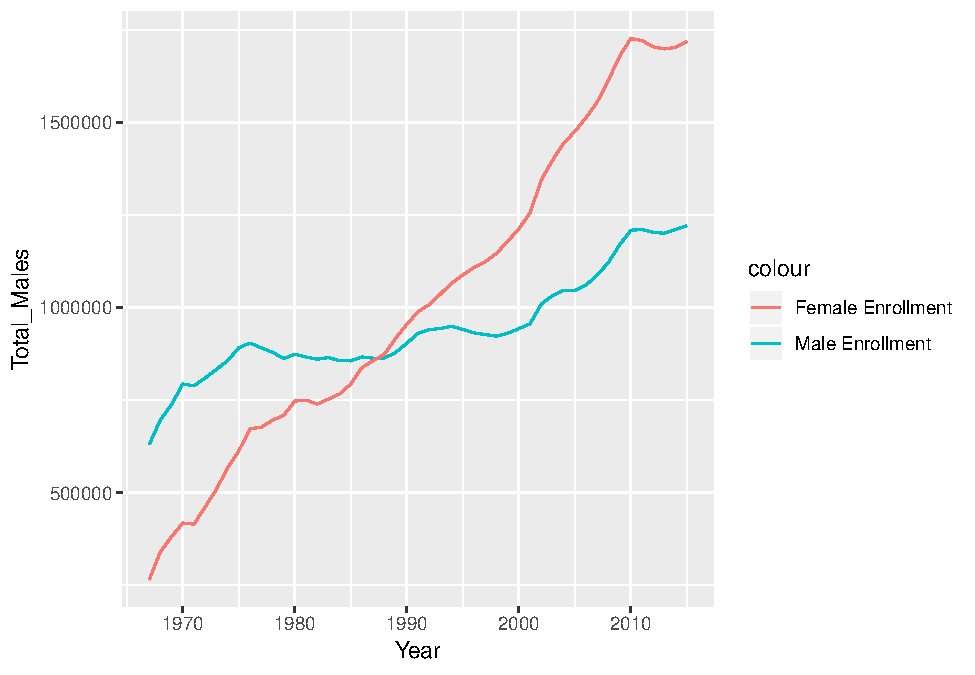
\includegraphics{Assignment_5_Markdown_files/figure-latex/unnamed-chunk-2-1.pdf}

\paragraph{Linear Regression for Male and Female
Enrollment}\label{linear-regression-for-male-and-female-enrollment}

\begin{Shaded}
\begin{Highlighting}[]
\NormalTok{menroll_model <-}\StringTok{ }\KeywordTok{lm}\NormalTok{(Total_Males }\OperatorTok{~}\StringTok{ }\NormalTok{Year, }\DataTypeTok{data =}\NormalTok{ enrollment)}
\NormalTok{menroll_model}
\end{Highlighting}
\end{Shaded}

\begin{verbatim}
## 
## Call:
## lm(formula = Total_Males ~ Year, data = enrollment)
## 
## Coefficients:
## (Intercept)         Year  
##   -17112153         9069
\end{verbatim}

\begin{Shaded}
\begin{Highlighting}[]
\CommentTok{#results in equation y = - 17112153 + 9069x}

\NormalTok{fenroll_model <-}\StringTok{ }\KeywordTok{lm}\NormalTok{(Total_Females }\OperatorTok{~}\StringTok{ }\NormalTok{Year, }\DataTypeTok{data =}\NormalTok{ enrollment)}
\NormalTok{fenroll_model}
\end{Highlighting}
\end{Shaded}

\begin{verbatim}
## 
## Call:
## lm(formula = Total_Females ~ Year, data = enrollment)
## 
## Coefficients:
## (Intercept)         Year  
##   -58955502        30126
\end{verbatim}

\begin{Shaded}
\begin{Highlighting}[]
\CommentTok{#results in equation y = - 58955502 + 30126x}
\end{Highlighting}
\end{Shaded}

\subparagraph{Model Diagnostics, Fit and
Significance}\label{model-diagnostics-fit-and-significance}

\begin{Shaded}
\begin{Highlighting}[]
\KeywordTok{plot}\NormalTok{(menroll_model)}
\end{Highlighting}
\end{Shaded}

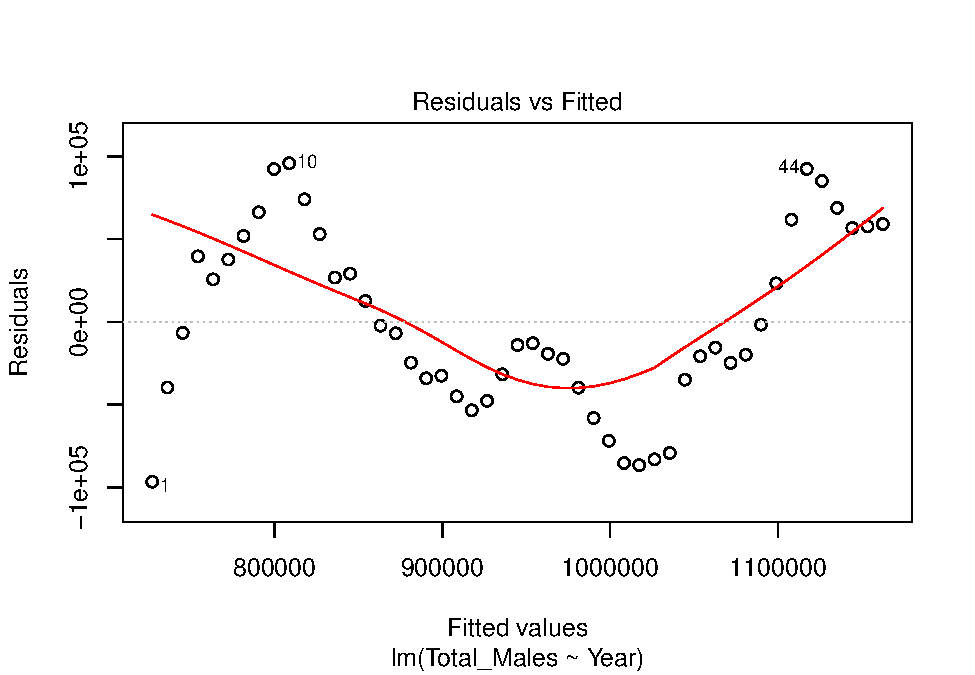
\includegraphics{Assignment_5_Markdown_files/figure-latex/unnamed-chunk-4-1.pdf}
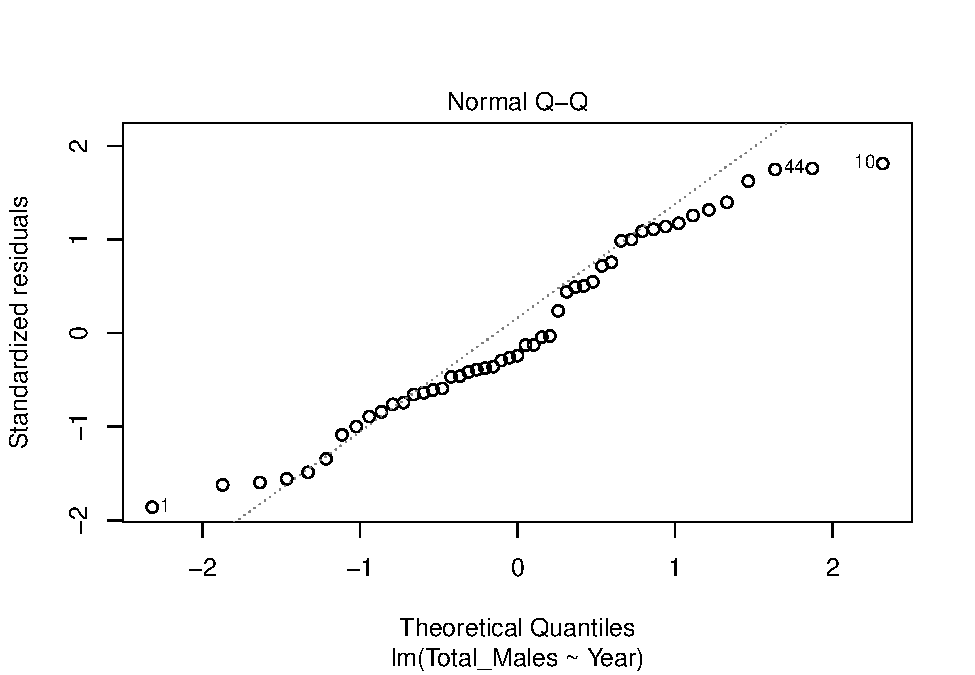
\includegraphics{Assignment_5_Markdown_files/figure-latex/unnamed-chunk-4-2.pdf}
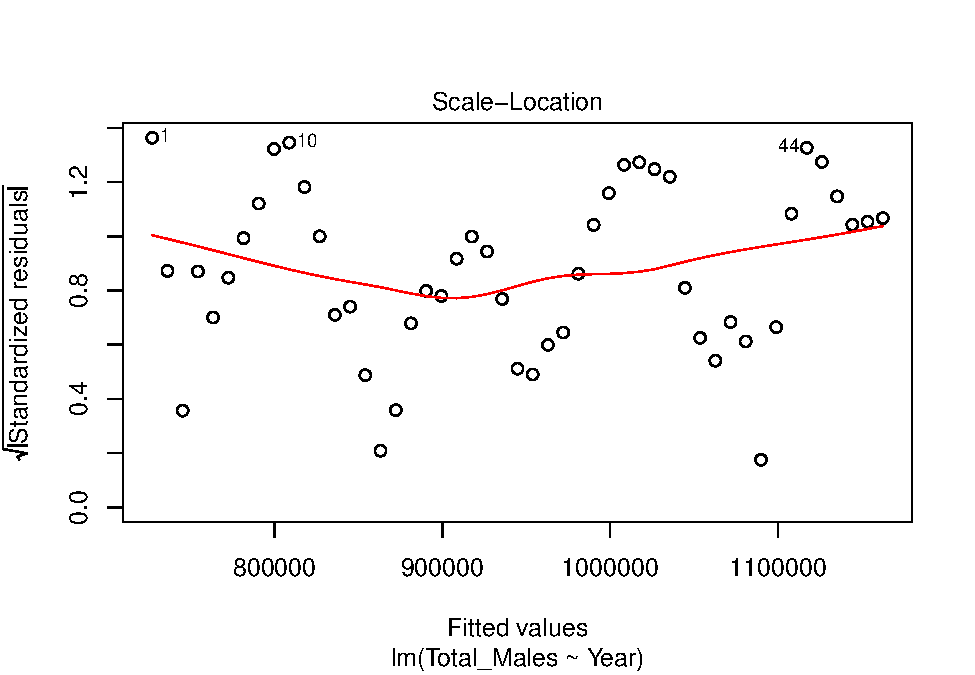
\includegraphics{Assignment_5_Markdown_files/figure-latex/unnamed-chunk-4-3.pdf}
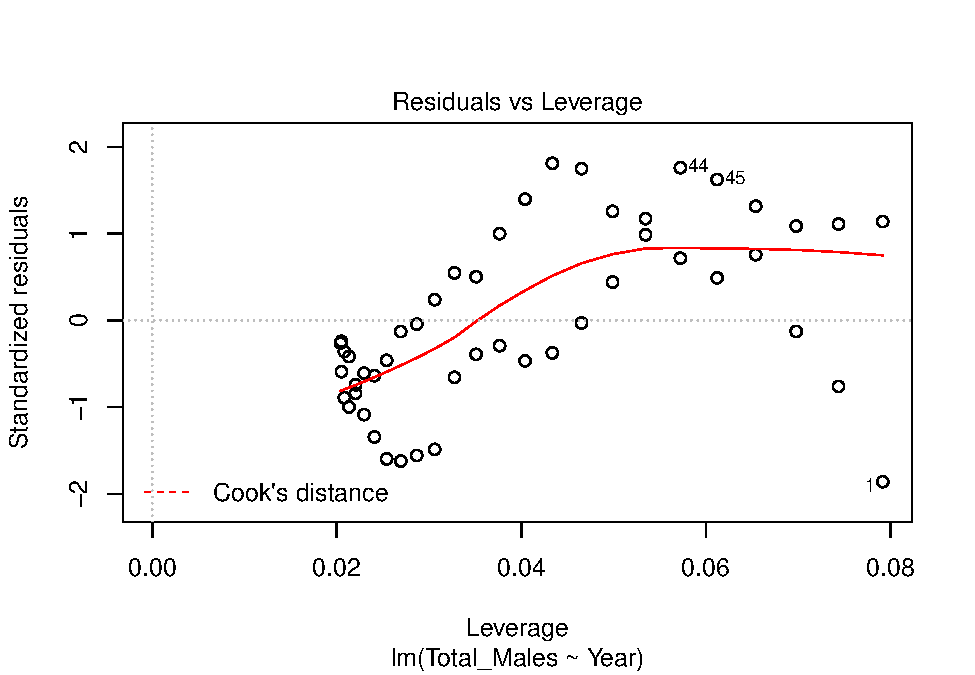
\includegraphics{Assignment_5_Markdown_files/figure-latex/unnamed-chunk-4-4.pdf}

\begin{Shaded}
\begin{Highlighting}[]
\KeywordTok{par}\NormalTok{(}\DataTypeTok{mfrow =} \KeywordTok{c}\NormalTok{(}\DecValTok{2}\NormalTok{,}\DecValTok{2}\NormalTok{))}
\KeywordTok{plot}\NormalTok{(menroll_model)}
\end{Highlighting}
\end{Shaded}

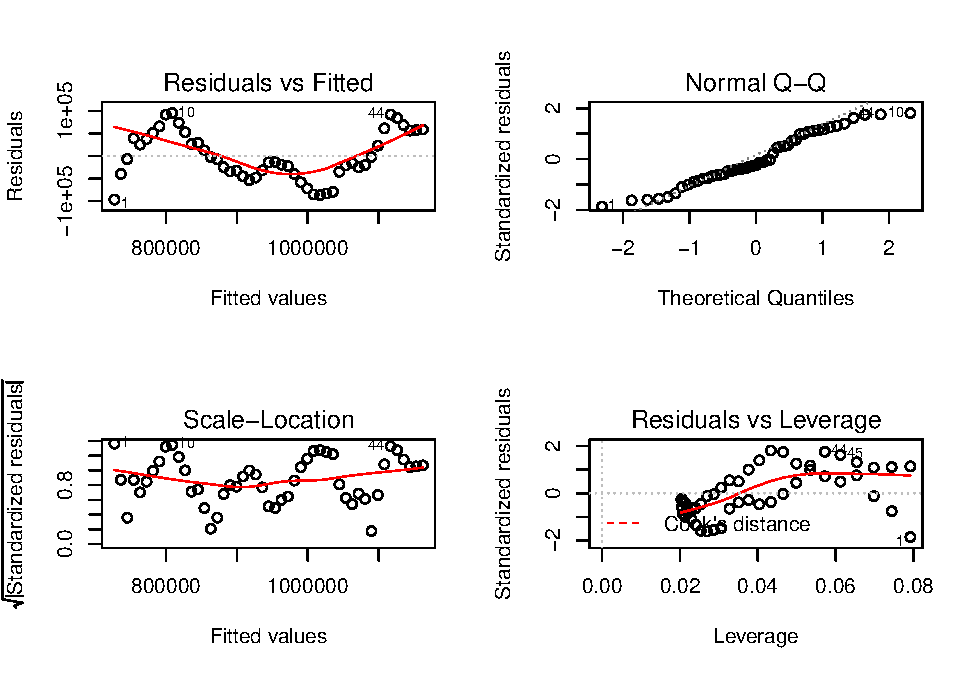
\includegraphics{Assignment_5_Markdown_files/figure-latex/unnamed-chunk-4-5.pdf}

\begin{Shaded}
\begin{Highlighting}[]
\CommentTok{#Q-Q plot appears normally distributed, but there seems to be peaks that don't match up with the red line on Residuals vs. Fitted graph.}

\KeywordTok{summary}\NormalTok{(menroll_model)}
\end{Highlighting}
\end{Shaded}

\begin{verbatim}
## 
## Call:
## lm(formula = Total_Males ~ Year, data = enrollment)
## 
## Residuals:
##    Min     1Q Median     3Q    Max 
## -96461 -34861 -12841  51876  95766 
## 
## Coefficients:
##              Estimate Std. Error t value Pr(>|t|)    
## (Intercept) -17112153    1087024  -15.74   <2e-16 ***
## Year             9069        546   16.61   <2e-16 ***
## ---
## Signif. codes:  0 '***' 0.001 '**' 0.01 '*' 0.05 '.' 0.1 ' ' 1
## 
## Residual standard error: 54050 on 47 degrees of freedom
## Multiple R-squared:  0.8545, Adjusted R-squared:  0.8514 
## F-statistic:   276 on 1 and 47 DF,  p-value: < 2.2e-16
\end{verbatim}

\begin{Shaded}
\begin{Highlighting}[]
\CommentTok{#Multiple R-squared:  0.8545,   Adjusted R-squared:  0.8514 }
\CommentTok{#F-statistic:   276 on 1 and 47 DF,  p-value: < 2.2e-16}
\CommentTok{#Standard error  1087024 and 546}

\KeywordTok{plot}\NormalTok{(fenroll_model)}
\KeywordTok{par}\NormalTok{(}\DataTypeTok{mfrow =} \KeywordTok{c}\NormalTok{(}\DecValTok{2}\NormalTok{,}\DecValTok{2}\NormalTok{))}
\KeywordTok{plot}\NormalTok{(fenroll_model)}
\end{Highlighting}
\end{Shaded}

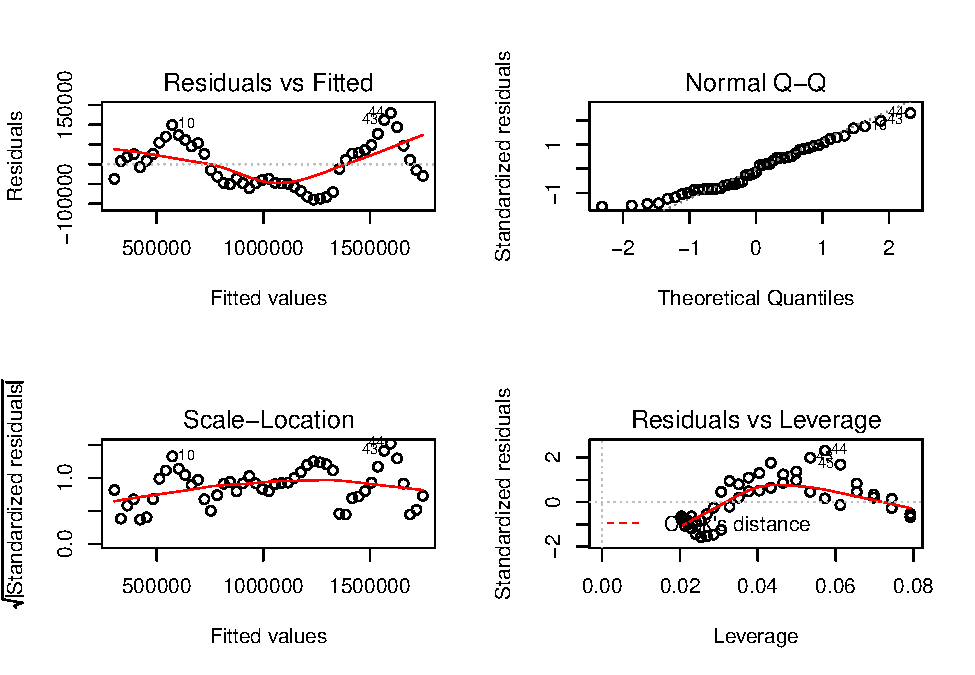
\includegraphics{Assignment_5_Markdown_files/figure-latex/unnamed-chunk-4-6.pdf}

\begin{Shaded}
\begin{Highlighting}[]
\CommentTok{#Q-Q plot appears normally distributed, but there seems to be peaks that don't match up with the red line on Residuals vs. Fitted graph.}

\KeywordTok{summary}\NormalTok{(fenroll_model)}
\end{Highlighting}
\end{Shaded}

\begin{verbatim}
## 
## Call:
## lm(formula = Total_Females ~ Year, data = enrollment)
## 
## Residuals:
##    Min     1Q Median     3Q    Max 
## -89397 -48101  -7633  45267 129727 
## 
## Coefficients:
##               Estimate Std. Error t value Pr(>|t|)    
## (Intercept) -5.896e+07  1.161e+06  -50.77   <2e-16 ***
## Year         3.013e+04  5.832e+02   51.66   <2e-16 ***
## ---
## Signif. codes:  0 '***' 0.001 '**' 0.01 '*' 0.05 '.' 0.1 ' ' 1
## 
## Residual standard error: 57730 on 47 degrees of freedom
## Multiple R-squared:  0.9827, Adjusted R-squared:  0.9823 
## F-statistic:  2669 on 1 and 47 DF,  p-value: < 2.2e-16
\end{verbatim}

\begin{Shaded}
\begin{Highlighting}[]
\CommentTok{#Multiple R-squared:  0.9827,   Adjusted R-squared:  0.9823 }
\CommentTok{#F-statistic:  2669 on 1 and 47 DF,  p-value: < 2.2e-16}
\CommentTok{#Standard error 1161000 and 583.2}
\end{Highlighting}
\end{Shaded}

\subparagraph{Finalized Graph for Male and Female
Enrollment}\label{finalized-graph-for-male-and-female-enrollment}

\begin{Shaded}
\begin{Highlighting}[]
\NormalTok{enrollment_graph <-}\StringTok{ }\KeywordTok{ggplot}\NormalTok{(enrollment, }\KeywordTok{aes}\NormalTok{(}\DataTypeTok{x=}\NormalTok{Year))}\OperatorTok{+}
\StringTok{  }\KeywordTok{geom_point}\NormalTok{(}\KeywordTok{aes}\NormalTok{(}\DataTypeTok{y=}\NormalTok{Total_Males}\OperatorTok{/}\DecValTok{1000000}\NormalTok{, }\DataTypeTok{color=}\StringTok{"Male"}\NormalTok{))}\OperatorTok{+}\StringTok{ }\CommentTok{#add cl smooth}
\StringTok{  }\KeywordTok{geom_point}\NormalTok{(}\KeywordTok{aes}\NormalTok{(}\DataTypeTok{y =}\NormalTok{ Total_Females}\OperatorTok{/}\DecValTok{1000000}\NormalTok{, }\DataTypeTok{color=}\StringTok{"Female"}\NormalTok{))}\OperatorTok{+}
\StringTok{  }\KeywordTok{geom_smooth}\NormalTok{(}\DataTypeTok{method =}\NormalTok{ lm, }\DataTypeTok{se =} \OtherTok{TRUE}\NormalTok{, }\DataTypeTok{size =} \FloatTok{0.5}\NormalTok{, }\DataTypeTok{color =} \StringTok{"midnightblue"}\NormalTok{,(}\KeywordTok{aes}\NormalTok{(}\DataTypeTok{y=}\NormalTok{Total_Males}\OperatorTok{/}\DecValTok{1000000}\NormalTok{)))}\OperatorTok{+}
\StringTok{  }\KeywordTok{geom_smooth}\NormalTok{(}\DataTypeTok{method =}\NormalTok{ lm, }\DataTypeTok{se =} \OtherTok{TRUE}\NormalTok{, }\DataTypeTok{size =} \FloatTok{0.5}\NormalTok{, }\DataTypeTok{color =} \StringTok{"orange1"}\NormalTok{,(}\KeywordTok{aes}\NormalTok{(}\DataTypeTok{y=}\NormalTok{Total_Females}\OperatorTok{/}\DecValTok{1000000}\NormalTok{)))}\OperatorTok{+}
\StringTok{  }\KeywordTok{theme_classic}\NormalTok{()}\OperatorTok{+}
\StringTok{  }\KeywordTok{scale_x_continuous}\NormalTok{(}\DataTypeTok{expand=} \KeywordTok{c}\NormalTok{(}\DecValTok{0}\NormalTok{,}\DecValTok{0}\NormalTok{), }\DataTypeTok{limits=} \KeywordTok{c}\NormalTok{(}\DecValTok{1967}\NormalTok{,}\DecValTok{2016}\NormalTok{))}\OperatorTok{+}
\StringTok{  }\KeywordTok{labs}\NormalTok{(}\DataTypeTok{x=} \StringTok{"Year"}\NormalTok{, }\DataTypeTok{y =} \StringTok{"Number of Students Enrolled (In Millions)"}\NormalTok{, }\DataTypeTok{color =} \StringTok{"Gender"}\NormalTok{)}

\NormalTok{enrollment_graph }\OperatorTok{+}\StringTok{ }\KeywordTok{scale_color_manual}\NormalTok{(}\DataTypeTok{values=}\KeywordTok{c}\NormalTok{(}\StringTok{"orange1"}\NormalTok{, }\StringTok{"midnightblue"}\NormalTok{))}
\end{Highlighting}
\end{Shaded}

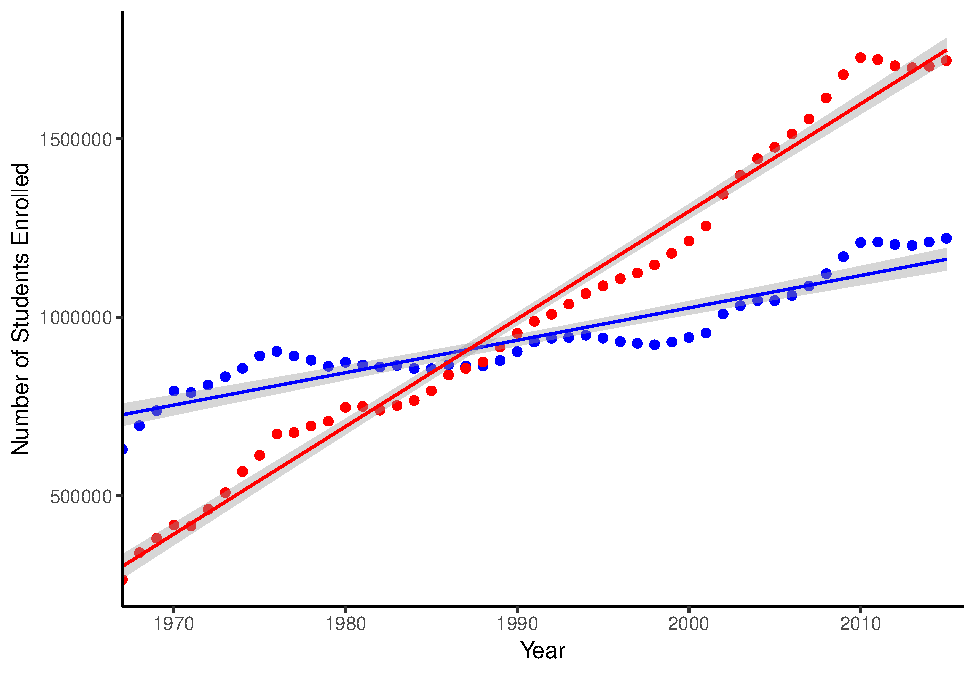
\includegraphics{Assignment_5_Markdown_files/figure-latex/unnamed-chunk-5-1.pdf}

\subsection{Part 2}\label{part-2}

\begin{Shaded}
\begin{Highlighting}[]
\CommentTok{#read csv file}
\NormalTok{phd <-}\StringTok{ }\KeywordTok{read_csv}\NormalTok{(}\StringTok{"phd.csv"}\NormalTok{) }
\end{Highlighting}
\end{Shaded}

\begin{verbatim}
## Parsed with column specification:
## cols(
##   `Field of Study` = col_character(),
##   field = col_character(),
##   sex = col_character(),
##   year = col_integer(),
##   number = col_number(),
##   percent = col_double()
## )
\end{verbatim}

\begin{Shaded}
\begin{Highlighting}[]
\NormalTok{ac_phd <-}\StringTok{ }\NormalTok{phd }\OperatorTok\StringTok{ }
\StringTok{  }\KeywordTok{filter}\NormalTok{(sex }\OperatorTok{==}\StringTok{ "female"}\NormalTok{) }\OperatorTok\StringTok{ }
\StringTok{  }\KeywordTok{filter}\NormalTok{(year }\OperatorTok{!=}\StringTok{ "1990"}\NormalTok{) }\OperatorTok\StringTok{ }
\StringTok{  }\KeywordTok{filter}\NormalTok{(year }\OperatorTok{!=}\StringTok{ "1995"}\NormalTok{) }\OperatorTok
\StringTok{  }\KeywordTok{filter}\NormalTok{(year }\OperatorTok{!=}\StringTok{ "2005"}\NormalTok{) }\OperatorTok\StringTok{ }
\StringTok{  }\KeywordTok{filter}\NormalTok{(year }\OperatorTok{!=}\StringTok{ "2010"}\NormalTok{) }\OperatorTok
\StringTok{  }\KeywordTok{filter}\NormalTok{(field }\OperatorTok{!=}\StringTok{ "all"}\NormalTok{) }\OperatorTok
\StringTok{  }\KeywordTok{filter}\NormalTok{(field }\OperatorTok{!=}\StringTok{ "lifesci"}\NormalTok{) }\OperatorTok
\StringTok{  }\KeywordTok{filter}\NormalTok{(field }\OperatorTok{!=}\StringTok{ "mathcomp"}\NormalTok{) }\OperatorTok
\StringTok{  }\KeywordTok{filter}\NormalTok{(field }\OperatorTok{!=}\StringTok{ "other"}\NormalTok{) }\OperatorTok
\StringTok{  }\KeywordTok{filter}\NormalTok{(field }\OperatorTok{!=}\StringTok{ "psychsoc"}\NormalTok{) }\OperatorTok\StringTok{ }
\StringTok{  }\KeywordTok{select}\NormalTok{(}\StringTok{"field"}\NormalTok{, }\StringTok{"sex"}\NormalTok{, }\StringTok{"year"}\NormalTok{, }\StringTok{"number"}\NormalTok{, }\StringTok{"percent"}\NormalTok{)}

\NormalTok{phd_prop <-}\StringTok{ }\NormalTok{ac_phd }\OperatorTok\StringTok{ }
\StringTok{  }\KeywordTok{select}\NormalTok{(}\StringTok{"field"}\NormalTok{, }\StringTok{"year"}\NormalTok{, }\StringTok{"number"}\NormalTok{) }

\NormalTok{phd_dcast <-}\StringTok{ }\KeywordTok{dcast}\NormalTok{(phd_prop, year}\OperatorTok{~}\NormalTok{field) }\OperatorTok\StringTok{ }
\StringTok{  }\KeywordTok{select}\NormalTok{(}\OperatorTok{-}\NormalTok{year)}
\end{Highlighting}
\end{Shaded}

\begin{verbatim}
## Using number as value column: use value.var to override.
\end{verbatim}

\begin{Shaded}
\begin{Highlighting}[]
\KeywordTok{rownames}\NormalTok{(phd_dcast) <-}\StringTok{ }\KeywordTok{c}\NormalTok{(}\StringTok{"1985"}\NormalTok{, }\StringTok{"2000"}\NormalTok{, }\StringTok{"2015"}\NormalTok{)}

\NormalTok{phd_proptable <-}\StringTok{ }\KeywordTok{prop.table}\NormalTok{(}\KeywordTok{as.matrix}\NormalTok{(phd_dcast),}\DecValTok{1}\NormalTok{)}

\NormalTok{female_phd_x2 <-}\StringTok{ }\KeywordTok{chisq.test}\NormalTok{(phd_dcast)}
\NormalTok{female_phd_x2}
\end{Highlighting}
\end{Shaded}

\begin{verbatim}
## 
##  Pearson's Chi-squared test
## 
## data:  phd_dcast
## X-squared = 2073.3, df = 6, p-value < 2.2e-16
\end{verbatim}

Pie chart for 1985

\begin{Shaded}
\begin{Highlighting}[]
\NormalTok{dfpie1985 <-}\StringTok{ }\KeywordTok{data.frame}\NormalTok{(}
  \DataTypeTok{group =} \KeywordTok{c}\NormalTok{(}\StringTok{"Education"}\NormalTok{, }\StringTok{"Engineering"}\NormalTok{, }\StringTok{"Humanities & Arts"}\NormalTok{, }\StringTok{"Physical & Earth Sciences"}\NormalTok{),}
  \DataTypeTok{value =} \KeywordTok{c}\NormalTok{(}\FloatTok{0.6178761}\NormalTok{, }\FloatTok{0.03504425}\NormalTok{, }\FloatTok{0.2463717}\NormalTok{, }\FloatTok{0.1007080}\NormalTok{)}
\NormalTok{  )}

\NormalTok{pie1985 <-}\StringTok{ }\KeywordTok{ggplot}\NormalTok{(dfpie1985, }\KeywordTok{aes}\NormalTok{(}\DataTypeTok{x=}\StringTok{""}\NormalTok{, }\DataTypeTok{y=}\NormalTok{value, }\DataTypeTok{fill=}\NormalTok{group)) }\OperatorTok{+}\StringTok{ }\KeywordTok{geom_bar}\NormalTok{(}\DataTypeTok{stat=}\StringTok{"identity"}\NormalTok{, }\DataTypeTok{width=}\DecValTok{1}\NormalTok{)}


\NormalTok{pie1985 =}\StringTok{ }\NormalTok{pie1985 }\OperatorTok{+}\StringTok{ }\KeywordTok{coord_polar}\NormalTok{(}\StringTok{"y"}\NormalTok{, }\DataTypeTok{start=}\DecValTok{0}\NormalTok{) }\OperatorTok{+}\StringTok{ }\KeywordTok{geom_text}\NormalTok{(}\KeywordTok{aes}\NormalTok{(}\DataTypeTok{label =} \KeywordTok{paste0}\NormalTok{(}\KeywordTok{round}\NormalTok{(value}\OperatorTok{*}\DecValTok{100}\NormalTok{), }\StringTok{"%"}\NormalTok{)), }\DataTypeTok{position =} \KeywordTok{position_stack}\NormalTok{(}\DataTypeTok{vjust =} \FloatTok{0.5}\NormalTok{))}

\NormalTok{pie1985 =}\StringTok{ }\NormalTok{pie1985 }\OperatorTok{+}\StringTok{ }\KeywordTok{scale_fill_manual}\NormalTok{(}\DataTypeTok{values=}\KeywordTok{c}\NormalTok{(}\StringTok{"#a3d9db"}\NormalTok{, }\StringTok{"#33658A"}\NormalTok{, }\StringTok{"#2F4858"}\NormalTok{, }\StringTok{"#e78f21"}\NormalTok{, }\StringTok{"#999999"}\NormalTok{))}

\NormalTok{pie1985 =}\StringTok{ }\NormalTok{pie1985 }\OperatorTok{+}\StringTok{ }\KeywordTok{theme_classic}\NormalTok{() }\OperatorTok{+}\StringTok{  }\KeywordTok{theme}\NormalTok{(}\DataTypeTok{legend.title=}\KeywordTok{element_blank}\NormalTok{())}\OperatorTok{+}\StringTok{ }\KeywordTok{labs}\NormalTok{(}\DataTypeTok{title =} \StringTok{"1985"}\NormalTok{, }\DataTypeTok{align=}\NormalTok{c)}\OperatorTok{+}\StringTok{ }\KeywordTok{theme}\NormalTok{(}\DataTypeTok{axis.line =} \KeywordTok{element_blank}\NormalTok{(),}
          \DataTypeTok{axis.text =} \KeywordTok{element_blank}\NormalTok{(),}
          \DataTypeTok{axis.ticks =} \KeywordTok{element_blank}\NormalTok{(),}
          \DataTypeTok{plot.title =} \KeywordTok{element_text}\NormalTok{(}\DataTypeTok{hjust =} \FloatTok{0.5}\NormalTok{, }\DataTypeTok{color =} \StringTok{"#666666"}\NormalTok{))}

\NormalTok{pie1985}
\end{Highlighting}
\end{Shaded}

\includegraphics{Assignment_5_Markdown_files/figure-latex/unnamed-chunk-7-1.pdf}

Pie chart for 2000

\begin{Shaded}
\begin{Highlighting}[]
\NormalTok{dfpie2000 <-}\StringTok{ }\KeywordTok{data.frame}\NormalTok{(}
  \DataTypeTok{group =} \KeywordTok{c}\NormalTok{(}\StringTok{"Education"}\NormalTok{, }\StringTok{"Engineering"}\NormalTok{, }\StringTok{"Humanities & Arts"}\NormalTok{, }\StringTok{"Physical & Earth Sciences"}\NormalTok{),}
  \DataTypeTok{value =} \KeywordTok{c}\NormalTok{(}\FloatTok{0.4797383}\NormalTok{, }\FloatTok{0.09620021}\NormalTok{, }\FloatTok{0.3067386}\NormalTok{, }\FloatTok{0.1173229}\NormalTok{)}
\NormalTok{  )}

\NormalTok{pie2000 <-}\StringTok{ }\KeywordTok{ggplot}\NormalTok{(dfpie2000, }\KeywordTok{aes}\NormalTok{(}\DataTypeTok{x=}\StringTok{""}\NormalTok{, }\DataTypeTok{y=}\NormalTok{value, }\DataTypeTok{fill=}\NormalTok{group)) }\OperatorTok{+}\StringTok{ }\KeywordTok{geom_bar}\NormalTok{(}\DataTypeTok{stat=}\StringTok{"identity"}\NormalTok{, }\DataTypeTok{width=}\DecValTok{1}\NormalTok{)}


\NormalTok{pie2000 =}\StringTok{ }\NormalTok{pie2000 }\OperatorTok{+}\StringTok{ }\KeywordTok{coord_polar}\NormalTok{(}\StringTok{"y"}\NormalTok{, }\DataTypeTok{start=}\DecValTok{0}\NormalTok{) }\OperatorTok{+}\StringTok{ }\KeywordTok{geom_text}\NormalTok{(}\KeywordTok{aes}\NormalTok{(}\DataTypeTok{label =} \KeywordTok{paste0}\NormalTok{(}\KeywordTok{round}\NormalTok{(value}\OperatorTok{*}\DecValTok{100}\NormalTok{), }\StringTok{"%"}\NormalTok{)), }\DataTypeTok{position =} \KeywordTok{position_stack}\NormalTok{(}\DataTypeTok{vjust =} \FloatTok{0.5}\NormalTok{))}

\NormalTok{pie2000 =}\StringTok{ }\NormalTok{pie2000 }\OperatorTok{+}\StringTok{ }\KeywordTok{scale_fill_manual}\NormalTok{(}\DataTypeTok{values=}\KeywordTok{c}\NormalTok{(}\StringTok{"#a3d9db"}\NormalTok{, }\StringTok{"#33658A"}\NormalTok{, }\StringTok{"#2F4858"}\NormalTok{, }\StringTok{"#e78f21"}\NormalTok{, }\StringTok{"#999999"}\NormalTok{))}

\NormalTok{pie2000 =}\StringTok{ }\NormalTok{pie2000 }\OperatorTok{+}\StringTok{ }\KeywordTok{theme_classic}\NormalTok{() }\OperatorTok{+}\StringTok{  }\KeywordTok{theme}\NormalTok{(}\DataTypeTok{legend.title=}\KeywordTok{element_blank}\NormalTok{())}\OperatorTok{+}\StringTok{ }\KeywordTok{labs}\NormalTok{(}\DataTypeTok{title =} \StringTok{"2000"}\NormalTok{, }\DataTypeTok{align=}\NormalTok{c)}\OperatorTok{+}\StringTok{ }\KeywordTok{theme}\NormalTok{(}\DataTypeTok{axis.line =} \KeywordTok{element_blank}\NormalTok{(),}
          \DataTypeTok{axis.text =} \KeywordTok{element_blank}\NormalTok{(),}
          \DataTypeTok{axis.ticks =} \KeywordTok{element_blank}\NormalTok{(),}
          \DataTypeTok{plot.title =} \KeywordTok{element_text}\NormalTok{(}\DataTypeTok{hjust =} \FloatTok{0.5}\NormalTok{, }\DataTypeTok{color =} \StringTok{"#666666"}\NormalTok{))}

\NormalTok{pie2000}
\end{Highlighting}
\end{Shaded}

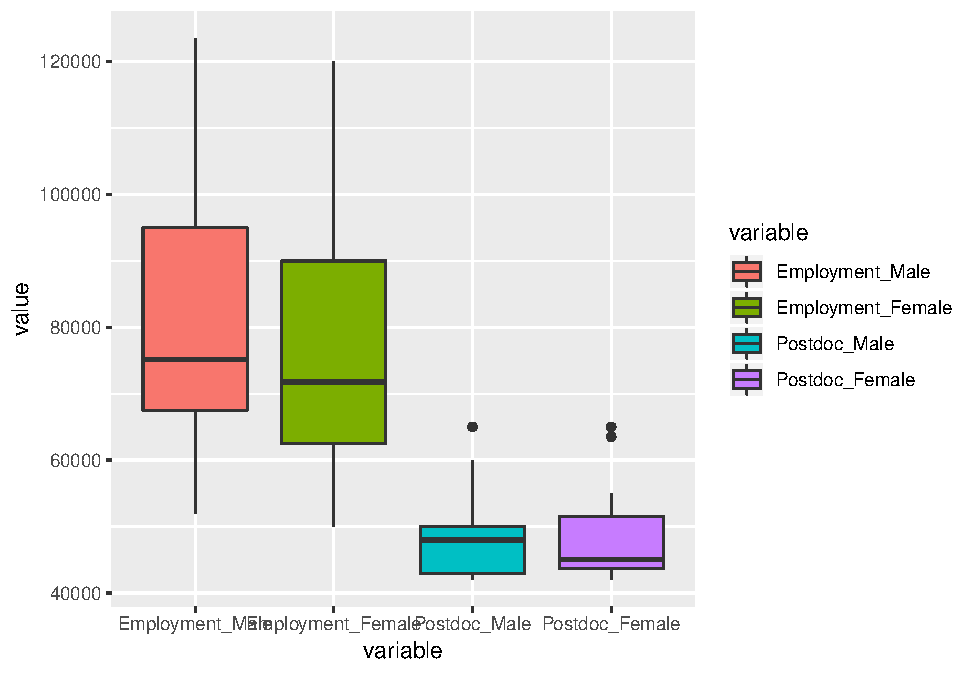
\includegraphics{Assignment_5_Markdown_files/figure-latex/unnamed-chunk-8-1.pdf}

Pie Chart for 2010

\begin{Shaded}
\begin{Highlighting}[]
\NormalTok{dfpie2015 <-}\StringTok{ }\KeywordTok{data.frame}\NormalTok{(}
  \DataTypeTok{group =} \KeywordTok{c}\NormalTok{(}\StringTok{"Education"}\NormalTok{, }\StringTok{"Engineering"}\NormalTok{, }\StringTok{"Humanities & Arts"}\NormalTok{, }\StringTok{"Physical & Earth Sciences"}\NormalTok{),}
  \DataTypeTok{value =} \KeywordTok{c}\NormalTok{(}\FloatTok{0.3296621}\NormalTok{, }\FloatTok{0.21660548}\NormalTok{, }\FloatTok{0.2665914}\NormalTok{, }\FloatTok{0.1871411}\NormalTok{)}
\NormalTok{  )}

\NormalTok{pie2015 <-}\StringTok{ }\KeywordTok{ggplot}\NormalTok{(dfpie2015, }\KeywordTok{aes}\NormalTok{(}\DataTypeTok{x=}\StringTok{""}\NormalTok{, }\DataTypeTok{y=}\NormalTok{value, }\DataTypeTok{fill=}\NormalTok{group)) }\OperatorTok{+}\StringTok{ }\KeywordTok{geom_bar}\NormalTok{(}\DataTypeTok{stat=}\StringTok{"identity"}\NormalTok{, }\DataTypeTok{width=}\DecValTok{1}\NormalTok{)}


\NormalTok{pie2015 =}\StringTok{ }\NormalTok{pie2015 }\OperatorTok{+}\StringTok{ }\KeywordTok{coord_polar}\NormalTok{(}\StringTok{"y"}\NormalTok{, }\DataTypeTok{start=}\DecValTok{0}\NormalTok{) }\OperatorTok{+}\StringTok{ }\KeywordTok{geom_text}\NormalTok{(}\KeywordTok{aes}\NormalTok{(}\DataTypeTok{label =} \KeywordTok{paste0}\NormalTok{(}\KeywordTok{round}\NormalTok{(value}\OperatorTok{*}\DecValTok{100}\NormalTok{), }\StringTok{"%"}\NormalTok{)), }\DataTypeTok{position =} \KeywordTok{position_stack}\NormalTok{(}\DataTypeTok{vjust =} \FloatTok{0.5}\NormalTok{))}

\NormalTok{pie2015 =}\StringTok{ }\NormalTok{pie2015 }\OperatorTok{+}\StringTok{ }\KeywordTok{scale_fill_manual}\NormalTok{(}\DataTypeTok{values=}\KeywordTok{c}\NormalTok{(}\StringTok{"#a3d9db"}\NormalTok{, }\StringTok{"#33658A"}\NormalTok{, }\StringTok{"#2F4858"}\NormalTok{, }\StringTok{"#e78f21"}\NormalTok{, }\StringTok{"#999999"}\NormalTok{))}

\NormalTok{pie2015 =}\StringTok{ }\NormalTok{pie2015 }\OperatorTok{+}\StringTok{ }\KeywordTok{theme_classic}\NormalTok{() }\OperatorTok{+}\StringTok{  }\KeywordTok{theme}\NormalTok{(}\DataTypeTok{legend.title=}\KeywordTok{element_blank}\NormalTok{())}\OperatorTok{+}\StringTok{ }\KeywordTok{labs}\NormalTok{(}\DataTypeTok{title =} \StringTok{"2015"}\NormalTok{, }\DataTypeTok{align=}\NormalTok{c)}\OperatorTok{+}\StringTok{ }\KeywordTok{theme}\NormalTok{(}\DataTypeTok{axis.line =} \KeywordTok{element_blank}\NormalTok{(),}
          \DataTypeTok{axis.text =} \KeywordTok{element_blank}\NormalTok{(),}
          \DataTypeTok{axis.ticks =} \KeywordTok{element_blank}\NormalTok{(),}
          \DataTypeTok{plot.title =} \KeywordTok{element_text}\NormalTok{(}\DataTypeTok{hjust =} \FloatTok{0.5}\NormalTok{, }\DataTypeTok{color =} \StringTok{"#666666"}\NormalTok{))}

\NormalTok{pie2015}
\end{Highlighting}
\end{Shaded}

\includegraphics{Assignment_5_Markdown_files/figure-latex/unnamed-chunk-9-1.pdf}

\section{Part 3 - Male and female salaries for starting postdoctoral and
other employment positions
(2015)}\label{part-3---male-and-female-salaries-for-starting-postdoctoral-and-other-employment-positions-2015}

Compare median salaries for male and female doctorate recipients in
2015. Answer these two questions:

Does median salary differ significantly between male and female starting
postdoc positions? Does median salary differ significantly between male
and female PhD recipients in non-postdoc employment positions?

Wilcoxon signed-rank - two sample paired

\begin{Shaded}
\begin{Highlighting}[]
\NormalTok{doctoral <-}\StringTok{ }\KeywordTok{read_csv}\NormalTok{(}\StringTok{"Doctoral_Salaries.csv"}\NormalTok{)}
\end{Highlighting}
\end{Shaded}

\begin{verbatim}
## Parsed with column specification:
## cols(
##   Field = col_character(),
##   Employment_Male = col_number(),
##   Employment_Female = col_number(),
##   Postdoc_Male = col_number(),
##   Postdoc_Female = col_number()
## )
\end{verbatim}

\subsection{Data visualization -
boxplots}\label{data-visualization---boxplots}

\begin{Shaded}
\begin{Highlighting}[]
\NormalTok{doctoral_melt <-}\StringTok{ }\KeywordTok{melt}\NormalTok{(doctoral[}\KeywordTok{c}\NormalTok{(}\StringTok{'Field'}\NormalTok{, }\StringTok{'Employment_Male'}\NormalTok{, }\StringTok{'Employment_Female'}\NormalTok{, }\StringTok{'Postdoc_Male'}\NormalTok{, }\StringTok{'Postdoc_Female'}\NormalTok{)],}\DataTypeTok{id.vars =} \DecValTok{1}\NormalTok{)}


\NormalTok{employment_box <-}\StringTok{ }\KeywordTok{ggplot}\NormalTok{(doctoral_melt, }\KeywordTok{aes}\NormalTok{(}\DataTypeTok{x =}\NormalTok{ variable, }\DataTypeTok{y =}\NormalTok{ value, }\DataTypeTok{fill =}\NormalTok{ variable))}\OperatorTok{+}
\StringTok{  }\KeywordTok{geom_boxplot}\NormalTok{()}
\NormalTok{employment_box}
\end{Highlighting}
\end{Shaded}

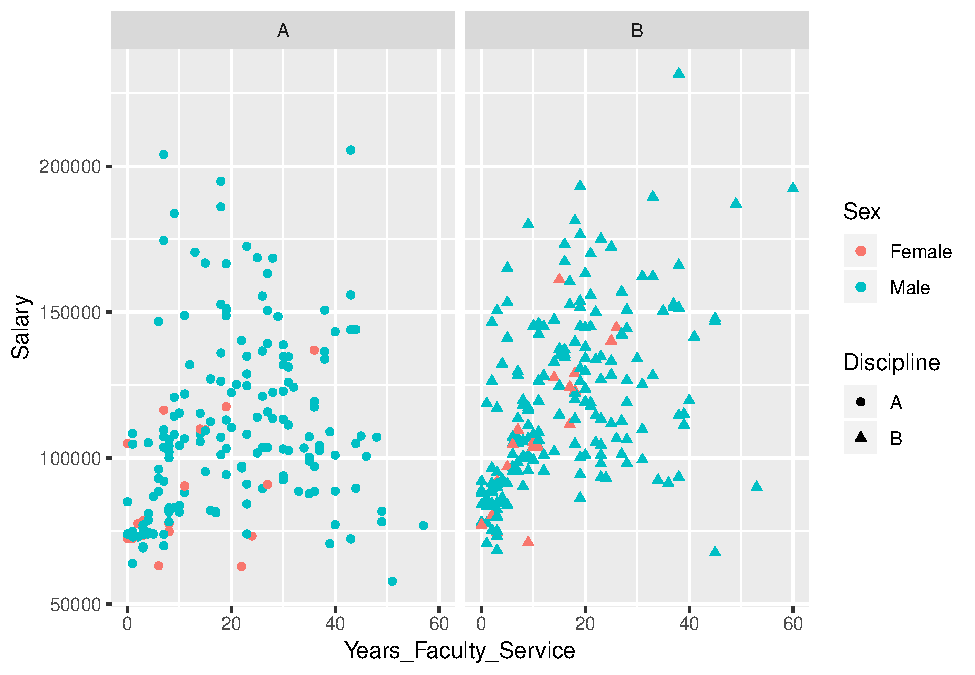
\includegraphics{Assignment_5_Markdown_files/figure-latex/unnamed-chunk-11-1.pdf}

\subsection{Wilcox rank test}\label{wilcox-rank-test}

\begin{Shaded}
\begin{Highlighting}[]
\NormalTok{employment_wilcox <-}\StringTok{ }\KeywordTok{wilcox.test}\NormalTok{(doctoral}\OperatorTok{$}\NormalTok{Employment_Male, doctoral}\OperatorTok{$}\NormalTok{Employment_Female, }\DataTypeTok{paired =} \OtherTok{TRUE}\NormalTok{)}
\end{Highlighting}
\end{Shaded}

\begin{verbatim}
## Warning in wilcox.test.default(doctoral$Employment_Male, doctoral
## $Employment_Female, : cannot compute exact p-value with ties
\end{verbatim}

\begin{verbatim}
## Warning in wilcox.test.default(doctoral$Employment_Male, doctoral
## $Employment_Female, : cannot compute exact p-value with zeroes
\end{verbatim}

\begin{Shaded}
\begin{Highlighting}[]
\NormalTok{employment_wilcox }\CommentTok{#V = 101, p-value = 0.002572}
\end{Highlighting}
\end{Shaded}

\begin{verbatim}
## 
##  Wilcoxon signed rank test with continuity correction
## 
## data:  doctoral$Employment_Male and doctoral$Employment_Female
## V = 101, p-value = 0.002572
## alternative hypothesis: true location shift is not equal to 0
\end{verbatim}

\begin{Shaded}
\begin{Highlighting}[]
\NormalTok{postdoc_wilcox <-}\StringTok{ }\KeywordTok{wilcox.test}\NormalTok{(doctoral}\OperatorTok{$}\NormalTok{Postdoc_Male, doctoral}\OperatorTok{$}\NormalTok{Postdoc_Female, }\DataTypeTok{paired =} \OtherTok{TRUE}\NormalTok{)}
\end{Highlighting}
\end{Shaded}

\begin{verbatim}
## Warning in wilcox.test.default(doctoral$Postdoc_Male, doctoral
## $Postdoc_Female, : cannot compute exact p-value with ties
\end{verbatim}

\begin{verbatim}
## Warning in wilcox.test.default(doctoral$Postdoc_Male, doctoral
## $Postdoc_Female, : cannot compute exact p-value with zeroes
\end{verbatim}

\begin{Shaded}
\begin{Highlighting}[]
\NormalTok{postdoc_wilcox }\CommentTok{#V = 19.5, p-value = 0.8884}
\end{Highlighting}
\end{Shaded}

\begin{verbatim}
## 
##  Wilcoxon signed rank test with continuity correction
## 
## data:  doctoral$Postdoc_Male and doctoral$Postdoc_Female
## V = 19.5, p-value = 0.8884
## alternative hypothesis: true location shift is not equal to 0
\end{verbatim}

\section{Part 4 - Multivariate linear
regression}\label{part-4---multivariate-linear-regression}

Exploring academic salaries for professors in U.S. colleges. Explore
relationships between variables in the `Faculty salary data (2008 - 2009
survey)' dataset. Develop a model describing faculty salary based on
data for faculty sex, rank, years in current position, field, and number
of years since doctoral degree was earned. You should make decisions
regarding which variables should remain in your final model. Describe
the results qualitatively and quantitatively (i.e., don't just report
the statistical results of the model -- make sure you describe
interesting findings in text). You can also discuss any concerns that
you have with the model(s) you present, if any.

Dependent variable (y): faculty salary Possible predictor variables:
faculty sex, rank, years in current position, field, and number of years
since doctoral degree was earned

Steps: 1) Explore data - find means of salary, make density plot of
salary by diff predictor variables 2) Make initial model 3) Test for
colinearity 4) Refine model 3) Run diagnostic plots (to test Linearity,
Independence, Homoscedasticity (residuals variance), Normality) 5) AIC
to compare different models

\subsection{Make new dataframe}\label{make-new-dataframe}

\begin{Shaded}
\begin{Highlighting}[]
\NormalTok{faculty_salary <-}\StringTok{ }\KeywordTok{read_csv}\NormalTok{(}\StringTok{"Faculty_Salaries.csv"}\NormalTok{)}
\end{Highlighting}
\end{Shaded}

\begin{verbatim}
## Parsed with column specification:
## cols(
##   Faculty_Rank = col_character(),
##   Discipline = col_character(),
##   Years_Since_PhD = col_integer(),
##   Years_Faculty_Service = col_integer(),
##   Sex = col_character(),
##   Salary = col_integer()
## )
\end{verbatim}

\begin{Shaded}
\begin{Highlighting}[]
\CommentTok{#Reorder columns}
\NormalTok{faculty_salary <-}\StringTok{ }\NormalTok{faculty_salary[}\KeywordTok{c}\NormalTok{(}\StringTok{"Salary"}\NormalTok{, }\StringTok{"Discipline"}\NormalTok{, }\StringTok{"Sex"}\NormalTok{, }\StringTok{"Faculty_Rank"}\NormalTok{, }\StringTok{"Years_Since_PhD"}\NormalTok{, }\StringTok{"Years_Faculty_Service"}\NormalTok{)]}
\end{Highlighting}
\end{Shaded}

\subsection{Explore data}\label{explore-data}

\begin{Shaded}
\begin{Highlighting}[]
\CommentTok{#Salary means by Sex}
\NormalTok{sex_mean <-}\StringTok{ }\NormalTok{faculty_salary }\OperatorTok\StringTok{ }
\StringTok{  }\KeywordTok{group_by}\NormalTok{(Sex) }\OperatorTok\StringTok{ }
\StringTok{  }\KeywordTok{summarize}\NormalTok{(}
    \DataTypeTok{mean =} \KeywordTok{mean}\NormalTok{(Salary)}
\NormalTok{  )}

\CommentTok{#Salary means by Discipline}
\NormalTok{discipline_mean <-}\StringTok{ }\NormalTok{faculty_salary }\OperatorTok\StringTok{ }
\StringTok{  }\KeywordTok{group_by}\NormalTok{(Discipline) }\OperatorTok\StringTok{ }
\StringTok{  }\KeywordTok{summarize}\NormalTok{(}
    \DataTypeTok{mean =} \KeywordTok{mean}\NormalTok{(Salary)}
\NormalTok{  )}

\CommentTok{#Relationship between salary and faculty years of service}
\NormalTok{salary_service <-}\StringTok{ }\KeywordTok{ggplot}\NormalTok{(faculty_salary, }\KeywordTok{aes}\NormalTok{(}\DataTypeTok{x =}\NormalTok{ Years_Faculty_Service, }\DataTypeTok{y =}\NormalTok{ Salary)) }\OperatorTok{+}
\StringTok{  }\KeywordTok{geom_point}\NormalTok{(}\KeywordTok{aes}\NormalTok{(}\DataTypeTok{color =}\NormalTok{ Sex, }\DataTypeTok{pch =}\NormalTok{ Discipline))}\OperatorTok{+}
\KeywordTok{facet_wrap}\NormalTok{(}\OperatorTok{~}\NormalTok{Discipline)}

\NormalTok{salary_service}
\end{Highlighting}
\end{Shaded}

\includegraphics{Assignment_5_Markdown_files/figure-latex/unnamed-chunk-14-1.pdf}

\begin{Shaded}
\begin{Highlighting}[]
\CommentTok{#Relationship between salary and faculty rank, by sex and discipline}
\NormalTok{salary_yrs <-}\StringTok{ }\KeywordTok{ggplot}\NormalTok{(faculty_salary, }\KeywordTok{aes}\NormalTok{(}\DataTypeTok{x =}\NormalTok{ Faculty_Rank, }\DataTypeTok{y =}\NormalTok{ Salary)) }\OperatorTok{+}
\StringTok{  }\KeywordTok{geom_point}\NormalTok{(}\KeywordTok{aes}\NormalTok{(}\DataTypeTok{color =}\NormalTok{ Sex, }\DataTypeTok{pch =}\NormalTok{ Discipline), }\DataTypeTok{alpha =} \FloatTok{0.5}\NormalTok{) }\OperatorTok{+}
\StringTok{  }\KeywordTok{facet_wrap}\NormalTok{(}\OperatorTok{~}\NormalTok{Discipline)}

\NormalTok{salary_yrs}
\end{Highlighting}
\end{Shaded}

\includegraphics{Assignment_5_Markdown_files/figure-latex/unnamed-chunk-14-2.pdf}

\subsection{Linear regression model - Saturated (all
variables)}\label{linear-regression-model---saturated-all-variables}

\begin{Shaded}
\begin{Highlighting}[]
\NormalTok{salary_lm1 <-}\StringTok{ }\KeywordTok{lm}\NormalTok{(Salary }\OperatorTok{~}\StringTok{ }\NormalTok{Discipline }\OperatorTok{+}\StringTok{ }\NormalTok{Sex }\OperatorTok{+}\StringTok{ }\NormalTok{Faculty_Rank }\OperatorTok{+}\StringTok{ }\NormalTok{Years_Since_PhD }\OperatorTok{+}\StringTok{ }\NormalTok{Years_Faculty_Service, }\DataTypeTok{data =}\NormalTok{ faculty_salary)}
\KeywordTok{summary}\NormalTok{(salary_lm1)}
\end{Highlighting}
\end{Shaded}

\begin{verbatim}
## 
## Call:
## lm(formula = Salary ~ Discipline + Sex + Faculty_Rank + Years_Since_PhD + 
##     Years_Faculty_Service, data = faculty_salary)
## 
## Residuals:
##    Min     1Q Median     3Q    Max 
## -65248 -13211  -1775  10384  99592 
## 
## Coefficients:
##                       Estimate Std. Error t value Pr(>|t|)    
## (Intercept)            78862.8     4990.3  15.803  < 2e-16 ***
## DisciplineB            14417.6     2342.9   6.154 1.88e-09 ***
## SexMale                 4783.5     3858.7   1.240  0.21584    
## Faculty_RankAsstProf  -12907.6     4145.3  -3.114  0.00198 ** 
## Faculty_RankProf       32158.4     3540.6   9.083  < 2e-16 ***
## Years_Since_PhD          535.1      241.0   2.220  0.02698 *  
## Years_Faculty_Service   -489.5      211.9  -2.310  0.02143 *  
## ---
## Signif. codes:  0 '***' 0.001 '**' 0.01 '*' 0.05 '.' 0.1 ' ' 1
## 
## Residual standard error: 22540 on 390 degrees of freedom
## Multiple R-squared:  0.4547, Adjusted R-squared:  0.4463 
## F-statistic:  54.2 on 6 and 390 DF,  p-value: < 2.2e-16
\end{verbatim}

Salary = 78862.8 + 14417.6(Discipline B) + 4783.5(Sex Male) -
12907.6(AsstProf) + 32158.4(Prof) + 535.1(Years\_Since\_PhD) - 489.5
(Years\_Faculty\_Service)

Reference levels: Discipline A (0), Female (0), AssocProf (0)

But\ldots{} this says that as you increase years of service, your salary
decreases -\textgreater{} Might indicate collinearity

\subsection{Test for collinearity}\label{test-for-collinearity}

\begin{Shaded}
\begin{Highlighting}[]
\NormalTok{salary_simple <-}\StringTok{ }\NormalTok{faculty_salary }\OperatorTok\StringTok{ }
\StringTok{  }\KeywordTok{select}\NormalTok{(Salary, Years_Since_PhD, Years_Faculty_Service)}

\KeywordTok{cor}\NormalTok{(salary_simple) }\CommentTok{#High correlation bw Years_Since_PhD and Years_Faculty_Service}
\end{Highlighting}
\end{Shaded}

\begin{verbatim}
##                          Salary Years_Since_PhD Years_Faculty_Service
## Salary                1.0000000       0.4192311             0.3347447
## Years_Since_PhD       0.4192311       1.0000000             0.9096491
## Years_Faculty_Service 0.3347447       0.9096491             1.0000000
\end{verbatim}

\begin{Shaded}
\begin{Highlighting}[]
\CommentTok{#VIF}
\KeywordTok{vif}\NormalTok{(salary_lm1)}
\end{Highlighting}
\end{Shaded}

\begin{verbatim}
##                           GVIF Df GVIF^(1/(2*Df))
## Discipline            1.064105  1        1.031555
## Sex                   1.030805  1        1.015285
## Faculty_Rank          2.013193  2        1.191163
## Years_Since_PhD       7.518936  1        2.742068
## Years_Faculty_Service 5.923038  1        2.433729
\end{verbatim}

High correlation bw Years\_Since\_PhD and Years\_Faculty\_Service: 0.91

VIF Years\_Since\_PhD: 7.51 Years\_Faculty\_Service: 5.92

So we should remove Years\_Since\_PhD or Years\_Faculty\_Service - which
makes sense conceptually

\subsection{Linear regression model -
subsets}\label{linear-regression-model---subsets}

\begin{Shaded}
\begin{Highlighting}[]
\CommentTok{#Model without Years_Since_PhD }
\NormalTok{salary_lm2 <-}\StringTok{ }\KeywordTok{lm}\NormalTok{(Salary }\OperatorTok{~}\StringTok{ }\NormalTok{Discipline }\OperatorTok{+}\StringTok{ }\NormalTok{Sex }\OperatorTok{+}\StringTok{ }\NormalTok{Faculty_Rank }\OperatorTok{+}\StringTok{ }\NormalTok{Years_Faculty_Service, }\DataTypeTok{data =}\NormalTok{ faculty_salary)}
\KeywordTok{summary}\NormalTok{(salary_lm2)}
\end{Highlighting}
\end{Shaded}

\begin{verbatim}
## 
## Call:
## lm(formula = Salary ~ Discipline + Sex + Faculty_Rank + Years_Faculty_Service, 
##     data = faculty_salary)
## 
## Residuals:
##    Min     1Q Median     3Q    Max 
## -64202 -14255  -1533  10571  99163 
## 
## Coefficients:
##                        Estimate Std. Error t value Pr(>|t|)    
## (Intercept)            82912.07    4668.39  17.760  < 2e-16 ***
## DisciplineB            13473.38    2315.50   5.819 1.24e-08 ***
## SexMale                 4771.25    3878.00   1.230 0.219311    
## Faculty_RankAsstProf  -14560.40    4098.32  -3.553 0.000428 ***
## Faculty_RankProf       34599.24    3382.52  10.229  < 2e-16 ***
## Years_Faculty_Service    -88.78     111.64  -0.795 0.426958    
## ---
## Signif. codes:  0 '***' 0.001 '**' 0.01 '*' 0.05 '.' 0.1 ' ' 1
## 
## Residual standard error: 22650 on 391 degrees of freedom
## Multiple R-squared:  0.4478, Adjusted R-squared:  0.4407 
## F-statistic: 63.41 on 5 and 391 DF,  p-value: < 2.2e-16
\end{verbatim}

\begin{Shaded}
\begin{Highlighting}[]
\KeywordTok{vif}\NormalTok{(salary_lm2)}
\end{Highlighting}
\end{Shaded}

\begin{verbatim}
##                           GVIF Df GVIF^(1/(2*Df))
## Discipline            1.029040  1        1.014416
## Sex                   1.030803  1        1.015284
## Faculty_Rank          1.597441  2        1.124233
## Years_Faculty_Service 1.627110  1        1.275582
\end{verbatim}

\begin{Shaded}
\begin{Highlighting}[]
\CommentTok{#Model without Years_Faculty_Service }
\NormalTok{salary_lm3 <-}\StringTok{ }\KeywordTok{lm}\NormalTok{(Salary }\OperatorTok{~}\StringTok{ }\NormalTok{Discipline }\OperatorTok{+}\StringTok{ }\NormalTok{Sex }\OperatorTok{+}\StringTok{ }\NormalTok{Faculty_Rank }\OperatorTok{+}\StringTok{ }\NormalTok{Years_Since_PhD, }\DataTypeTok{data =}\NormalTok{ faculty_salary)}
\KeywordTok{summary}\NormalTok{(salary_lm3)}
\end{Highlighting}
\end{Shaded}

\begin{verbatim}
## 
## Call:
## lm(formula = Salary ~ Discipline + Sex + Faculty_Rank + Years_Since_PhD, 
##     data = faculty_salary)
## 
## Residuals:
##    Min     1Q Median     3Q    Max 
## -67451 -13860  -1549  10716  97023 
## 
## Coefficients:
##                       Estimate Std. Error t value Pr(>|t|)    
## (Intercept)           80988.47    4931.84  16.422  < 2e-16 ***
## DisciplineB           13937.47    2346.53   5.940 6.32e-09 ***
## SexMale                4349.37    3875.39   1.122  0.26242    
## Faculty_RankAsstProf -13104.15    4167.31  -3.145  0.00179 ** 
## Faculty_RankProf      32928.40    3544.40   9.290  < 2e-16 ***
## Years_Since_PhD          61.01     127.01   0.480  0.63124    
## ---
## Signif. codes:  0 '***' 0.001 '**' 0.01 '*' 0.05 '.' 0.1 ' ' 1
## 
## Residual standard error: 22660 on 391 degrees of freedom
## Multiple R-squared:  0.4472, Adjusted R-squared:  0.4401 
## F-statistic: 63.27 on 5 and 391 DF,  p-value: < 2.2e-16
\end{verbatim}

\begin{Shaded}
\begin{Highlighting}[]
\KeywordTok{vif}\NormalTok{(salary_lm3)}
\end{Highlighting}
\end{Shaded}

\begin{verbatim}
##                     GVIF Df GVIF^(1/(2*Df))
## Discipline      1.055727  1        1.027486
## Sex             1.028359  1        1.014080
## Faculty_Rank    1.987205  2        1.187301
## Years_Since_PhD 2.065517  1        1.437191
\end{verbatim}

\begin{Shaded}
\begin{Highlighting}[]
\CommentTok{#Model without Years_Since_PhD and Years_Faculty_Service}
\NormalTok{salary_lm4 <-}\StringTok{ }\KeywordTok{lm}\NormalTok{(Salary }\OperatorTok{~}\StringTok{ }\NormalTok{Discipline }\OperatorTok{+}\StringTok{ }\NormalTok{Sex }\OperatorTok{+}\StringTok{ }\NormalTok{Faculty_Rank, }\DataTypeTok{data =}\NormalTok{ faculty_salary)}
\KeywordTok{summary}\NormalTok{(salary_lm4)}
\end{Highlighting}
\end{Shaded}

\begin{verbatim}
## 
## Call:
## lm(formula = Salary ~ Discipline + Sex + Faculty_Rank, data = faculty_salary)
## 
## Residuals:
##    Min     1Q Median     3Q    Max 
## -66268 -14127  -1566  10813  97718 
## 
## Coefficients:
##                      Estimate Std. Error t value Pr(>|t|)    
## (Intercept)             81947       4506  18.187  < 2e-16 ***
## DisciplineB             13709       2295   5.972 5.25e-09 ***
## SexMale                  4492       3860   1.164 0.245291    
## Faculty_RankAsstProf   -13723       3959  -3.466 0.000586 ***
## Faculty_RankProf        33680       3177  10.600  < 2e-16 ***
## ---
## Signif. codes:  0 '***' 0.001 '**' 0.01 '*' 0.05 '.' 0.1 ' ' 1
## 
## Residual standard error: 22640 on 392 degrees of freedom
## Multiple R-squared:  0.4469, Adjusted R-squared:  0.4412 
## F-statistic: 79.18 on 4 and 392 DF,  p-value: < 2.2e-16
\end{verbatim}

\begin{Shaded}
\begin{Highlighting}[]
\KeywordTok{vif}\NormalTok{(salary_lm4)}
\end{Highlighting}
\end{Shaded}

\begin{verbatim}
##                  GVIF Df GVIF^(1/(2*Df))
## Discipline   1.012236  1        1.006099
## Sex          1.022339  1        1.011108
## Faculty_Rank 1.034437  2        1.008500
\end{verbatim}

Model lm2 (Model without Years\_Since\_PhD): Salary = 82912.1 +
13473.4(Discipline B) + 4771.3(Sex Male) - 14560.4(AsstProf) +
34599.2(Prof) - 88.8 (Years\_Faculty\_Service)

Model lm3 (Model without Years\_Faculty\_Service): Salary = 80988.5 +
13937.5(Discipline B) + 4349.4(Sex Male) - 13104.2(AsstProf) +
32928.4(Prof) + 61.0 (Years\_Since\_PhD)

Model lm4: Salary = 81947 + 13709(Discipline B) + 4492(Sex Male) -
13723(AsstProf) + 33680(Prof)

\subsection{Interaction terms?}\label{interaction-terms}

\begin{Shaded}
\begin{Highlighting}[]
\NormalTok{salary_lm5 <-}\StringTok{ }\KeywordTok{lm}\NormalTok{(Salary }\OperatorTok{~}\StringTok{ }\NormalTok{Sex }\OperatorTok{+}\StringTok{ }\NormalTok{Faculty_Rank }\OperatorTok{+}\StringTok{ }\NormalTok{Discipline }\OperatorTok{+}\StringTok{ }\NormalTok{Years_Faculty_Service }\OperatorTok{+}\StringTok{ }\NormalTok{Discipline}\OperatorTok{*}\NormalTok{Years_Faculty_Service, }\DataTypeTok{data =}\NormalTok{ faculty_salary)}

\KeywordTok{summary}\NormalTok{(salary_lm5)}
\end{Highlighting}
\end{Shaded}

\begin{verbatim}
## 
## Call:
## lm(formula = Salary ~ Sex + Faculty_Rank + Discipline + Years_Faculty_Service + 
##     Discipline * Years_Faculty_Service, data = faculty_salary)
## 
## Residuals:
##    Min     1Q Median     3Q    Max 
## -70632 -14191  -2098   9937  94331 
## 
## Coefficients:
##                                   Estimate Std. Error t value Pr(>|t|)    
## (Intercept)                        86338.5     4880.9  17.689  < 2e-16 ***
## SexMale                             5196.1     3861.9   1.345 0.179254    
## Faculty_RankAsstProf              -13899.7     4086.8  -3.401 0.000741 ***
## Faculty_RankProf                   34121.8     3371.0  10.122  < 2e-16 ***
## DisciplineB                         6255.7     3916.2   1.597 0.110989    
## Years_Faculty_Service               -266.8      135.8  -1.965 0.050128 .  
## DisciplineB:Years_Faculty_Service    406.3      178.3   2.279 0.023221 *  
## ---
## Signif. codes:  0 '***' 0.001 '**' 0.01 '*' 0.05 '.' 0.1 ' ' 1
## 
## Residual standard error: 22530 on 390 degrees of freedom
## Multiple R-squared:  0.455,  Adjusted R-squared:  0.4467 
## F-statistic: 54.27 on 6 and 390 DF,  p-value: < 2.2e-16
\end{verbatim}

\begin{Shaded}
\begin{Highlighting}[]
\KeywordTok{vif}\NormalTok{(salary_lm5)}
\end{Highlighting}
\end{Shaded}

\begin{verbatim}
##                                      GVIF Df GVIF^(1/(2*Df))
## Sex                              1.033210  1        1.016469
## Faculty_Rank                     1.625251  2        1.129094
## Discipline                       2.975161  1        1.724865
## Years_Faculty_Service            2.432170  1        1.559542
## Discipline:Years_Faculty_Service 3.484050  1        1.866561
\end{verbatim}

\begin{Shaded}
\begin{Highlighting}[]
\CommentTok{#Relationship between salary and Years_Faculty_Service, by discipline}
\NormalTok{service_model <-}\StringTok{ }\KeywordTok{lm}\NormalTok{(Salary }\OperatorTok{~}\StringTok{ }\NormalTok{Years_Faculty_Service }\OperatorTok{+}\StringTok{ }\NormalTok{Discipline, }\DataTypeTok{data =}\NormalTok{ faculty_salary)}

\NormalTok{service_graph1 <-}\StringTok{ }\KeywordTok{ggplot}\NormalTok{(faculty_salary, }\KeywordTok{aes}\NormalTok{(}\DataTypeTok{x =}\NormalTok{ Years_Faculty_Service, }\DataTypeTok{y =}\NormalTok{ Salary))}\OperatorTok{+}
\KeywordTok{geom_point}\NormalTok{(}\KeywordTok{aes}\NormalTok{(}\DataTypeTok{color =}\NormalTok{ Discipline))}\OperatorTok{+}
\StringTok{  }\KeywordTok{facet_wrap}\NormalTok{(}\OperatorTok{~}\NormalTok{Discipline)}\OperatorTok{+}
\StringTok{  }\KeywordTok{geom_smooth}\NormalTok{(}\DataTypeTok{method =}\NormalTok{ lm, }\DataTypeTok{se =} \OtherTok{TRUE}\NormalTok{, }\DataTypeTok{size =} \FloatTok{0.5}\NormalTok{, }\DataTypeTok{color =} \StringTok{"gray20"}\NormalTok{)}
\NormalTok{service_graph1}
\end{Highlighting}
\end{Shaded}

\includegraphics{Assignment_5_Markdown_files/figure-latex/unnamed-chunk-18-1.pdf}

\begin{Shaded}
\begin{Highlighting}[]
\NormalTok{service_graph2 <-}\StringTok{ }\KeywordTok{ggplot}\NormalTok{(faculty_salary, }\KeywordTok{aes}\NormalTok{(}\DataTypeTok{x =}\NormalTok{ Years_Faculty_Service, }\DataTypeTok{y =}\NormalTok{ Salary))}\OperatorTok{+}
\KeywordTok{geom_point}\NormalTok{()}\OperatorTok{+}
\StringTok{  }\KeywordTok{geom_smooth}\NormalTok{(}\DataTypeTok{method =}\NormalTok{ lm, }\DataTypeTok{se =} \OtherTok{TRUE}\NormalTok{, }\DataTypeTok{size =} \FloatTok{0.5}\NormalTok{, }\DataTypeTok{color =} \StringTok{"gray20"}\NormalTok{)}
\NormalTok{service_graph2}
\end{Highlighting}
\end{Shaded}

\includegraphics{Assignment_5_Markdown_files/figure-latex/unnamed-chunk-18-2.pdf}

\begin{Shaded}
\begin{Highlighting}[]
\NormalTok{service_graph3 <-}\StringTok{ }\KeywordTok{ggplot}\NormalTok{(faculty_salary, }\KeywordTok{aes}\NormalTok{(}\DataTypeTok{x =}\NormalTok{ Years_Since_PhD, }\DataTypeTok{y =}\NormalTok{ Salary))}\OperatorTok{+}
\KeywordTok{geom_point}\NormalTok{()}\OperatorTok{+}
\StringTok{  }\KeywordTok{geom_smooth}\NormalTok{(}\DataTypeTok{method =}\NormalTok{ lm, }\DataTypeTok{se =} \OtherTok{TRUE}\NormalTok{, }\DataTypeTok{size =} \FloatTok{0.5}\NormalTok{, }\DataTypeTok{color =} \StringTok{"gray20"}\NormalTok{)}
\NormalTok{service_graph3}
\end{Highlighting}
\end{Shaded}

\includegraphics{Assignment_5_Markdown_files/figure-latex/unnamed-chunk-18-3.pdf}

\subsection{Diagnostic plots}\label{diagnostic-plots}

\begin{Shaded}
\begin{Highlighting}[]
\KeywordTok{plot}\NormalTok{(salary_lm2)}
\end{Highlighting}
\end{Shaded}

\includegraphics{Assignment_5_Markdown_files/figure-latex/unnamed-chunk-19-1.pdf}
\includegraphics{Assignment_5_Markdown_files/figure-latex/unnamed-chunk-19-2.pdf}
\includegraphics{Assignment_5_Markdown_files/figure-latex/unnamed-chunk-19-3.pdf}
\includegraphics{Assignment_5_Markdown_files/figure-latex/unnamed-chunk-19-4.pdf}

\begin{Shaded}
\begin{Highlighting}[]
\KeywordTok{plot}\NormalTok{(salary_lm3)}
\end{Highlighting}
\end{Shaded}

\includegraphics{Assignment_5_Markdown_files/figure-latex/unnamed-chunk-19-5.pdf}
\includegraphics{Assignment_5_Markdown_files/figure-latex/unnamed-chunk-19-6.pdf}
\includegraphics{Assignment_5_Markdown_files/figure-latex/unnamed-chunk-19-7.pdf}
\includegraphics{Assignment_5_Markdown_files/figure-latex/unnamed-chunk-19-8.pdf}

\begin{Shaded}
\begin{Highlighting}[]
\KeywordTok{plot}\NormalTok{(salary_lm4)}
\end{Highlighting}
\end{Shaded}

\includegraphics{Assignment_5_Markdown_files/figure-latex/unnamed-chunk-19-9.pdf}
\includegraphics{Assignment_5_Markdown_files/figure-latex/unnamed-chunk-19-10.pdf}
\includegraphics{Assignment_5_Markdown_files/figure-latex/unnamed-chunk-19-11.pdf}
\includegraphics{Assignment_5_Markdown_files/figure-latex/unnamed-chunk-19-12.pdf}

\begin{Shaded}
\begin{Highlighting}[]
\KeywordTok{plot}\NormalTok{(salary_lm5)}
\end{Highlighting}
\end{Shaded}

\includegraphics{Assignment_5_Markdown_files/figure-latex/unnamed-chunk-19-13.pdf}
\includegraphics{Assignment_5_Markdown_files/figure-latex/unnamed-chunk-19-14.pdf}
\includegraphics{Assignment_5_Markdown_files/figure-latex/unnamed-chunk-19-15.pdf}
\includegraphics{Assignment_5_Markdown_files/figure-latex/unnamed-chunk-19-16.pdf}
Residuals: homoscedastic?? Normality: yes??

\subsection{Akaike Information
Criterion}\label{akaike-information-criterion}

\begin{Shaded}
\begin{Highlighting}[]
\NormalTok{sat_aic <-}\StringTok{ }\KeywordTok{AIC}\NormalTok{(salary_lm1)}
\NormalTok{sat_aic }\CommentTok{#9093.8}
\end{Highlighting}
\end{Shaded}

\begin{verbatim}
## [1] 9093.826
\end{verbatim}

\begin{Shaded}
\begin{Highlighting}[]
\NormalTok{lm2_aic <-}\StringTok{ }\KeywordTok{AIC}\NormalTok{(salary_lm2)}
\NormalTok{lm2_aic }\CommentTok{#9096.8}
\end{Highlighting}
\end{Shaded}

\begin{verbatim}
## [1] 9096.813
\end{verbatim}

\begin{Shaded}
\begin{Highlighting}[]
\NormalTok{lm3_aic <-}\StringTok{ }\KeywordTok{AIC}\NormalTok{(salary_lm3)}
\NormalTok{lm3_aic }\CommentTok{#9097.2}
\end{Highlighting}
\end{Shaded}

\begin{verbatim}
## [1] 9097.22
\end{verbatim}

\begin{Shaded}
\begin{Highlighting}[]
\NormalTok{lm4_aic <-}\StringTok{ }\KeywordTok{AIC}\NormalTok{(salary_lm4)}
\NormalTok{lm4_aic }\CommentTok{#9095.5}
\end{Highlighting}
\end{Shaded}

\begin{verbatim}
## [1] 9095.454
\end{verbatim}

\begin{Shaded}
\begin{Highlighting}[]
\NormalTok{lm5_aic <-}\StringTok{ }\KeywordTok{AIC}\NormalTok{(salary_lm5)}
\NormalTok{lm5_aic }\CommentTok{#9093.6}
\end{Highlighting}
\end{Shaded}

\begin{verbatim}
## [1] 9093.562
\end{verbatim}

\begin{Shaded}
\begin{Highlighting}[]
\CommentTok{#lm4 < lm3 < lm2}
\end{Highlighting}
\end{Shaded}

None of the interactions significantly change the AIC value of the
model. SO: The best model is lm3

Model lm3 (Model without Years\_Faculty\_Service): Salary = 80988.5 +
13937.5(Discipline B) + 4349.4(Sex Male) - 13104.2(AsstProf) +
32928.4(Prof) + 61.0 (Years\_Since\_PhD)

\subsection{Model data table}\label{model-data-table}

\begin{Shaded}
\begin{Highlighting}[]
\NormalTok{lm_table <-}\StringTok{ }\KeywordTok{stargazer}\NormalTok{(salary_lm3, }\DataTypeTok{type =} \StringTok{"html"}\NormalTok{)}
\end{Highlighting}
\end{Shaded}

\begin{verbatim}
## 
## <table style="text-align:center"><tr><td colspan="2" style="border-bottom: 1px solid black"></td></tr><tr><td style="text-align:left"></td><td><em>Dependent variable:</em></td></tr>
## <tr><td></td><td colspan="1" style="border-bottom: 1px solid black"></td></tr>
## <tr><td style="text-align:left"></td><td>Salary</td></tr>
## <tr><td colspan="2" style="border-bottom: 1px solid black"></td></tr><tr><td style="text-align:left">DisciplineB</td><td>13,937.470<sup>***</sup></td></tr>
## <tr><td style="text-align:left"></td><td>(2,346.534)</td></tr>
## <tr><td style="text-align:left"></td><td></td></tr>
## <tr><td style="text-align:left">SexMale</td><td>4,349.366</td></tr>
## <tr><td style="text-align:left"></td><td>(3,875.393)</td></tr>
## <tr><td style="text-align:left"></td><td></td></tr>
## <tr><td style="text-align:left">Faculty_RankAsstProf</td><td>-13,104.150<sup>***</sup></td></tr>
## <tr><td style="text-align:left"></td><td>(4,167.315)</td></tr>
## <tr><td style="text-align:left"></td><td></td></tr>
## <tr><td style="text-align:left">Faculty_RankProf</td><td>32,928.400<sup>***</sup></td></tr>
## <tr><td style="text-align:left"></td><td>(3,544.403)</td></tr>
## <tr><td style="text-align:left"></td><td></td></tr>
## <tr><td style="text-align:left">Years_Since_PhD</td><td>61.011</td></tr>
## <tr><td style="text-align:left"></td><td>(127.010)</td></tr>
## <tr><td style="text-align:left"></td><td></td></tr>
## <tr><td style="text-align:left">Constant</td><td>80,988.470<sup>***</sup></td></tr>
## <tr><td style="text-align:left"></td><td>(4,931.844)</td></tr>
## <tr><td style="text-align:left"></td><td></td></tr>
## <tr><td colspan="2" style="border-bottom: 1px solid black"></td></tr><tr><td style="text-align:left">Observations</td><td>397</td></tr>
## <tr><td style="text-align:left">R<sup>2</sup></td><td>0.447</td></tr>
## <tr><td style="text-align:left">Adjusted R<sup>2</sup></td><td>0.440</td></tr>
## <tr><td style="text-align:left">Residual Std. Error</td><td>22,663.240 (df = 391)</td></tr>
## <tr><td style="text-align:left">F Statistic</td><td>63.266<sup>***</sup> (df = 5; 391)</td></tr>
## <tr><td colspan="2" style="border-bottom: 1px solid black"></td></tr><tr><td style="text-align:left"><em>Note:</em></td><td style="text-align:right"><sup>*</sup>p<0.1; <sup>**</sup>p<0.05; <sup>***</sup>p<0.01</td></tr>
## </table>
\end{verbatim}


\end{document}
